%!TEX TS-program = xelatex
\documentclass[aspectratio=169,newPxFont]{beamer}
%\documentclass[newPxFont,handout]{beamer} % Раздаточный материал (на слайдах всё сразу)
%\documentclass[aspectratio=169]{beamer} % Соотношение сторон

\usetheme{LTX}

%-=-=-=-=-=-=-=-=-=-=-=-=-=-=-=-=-=-=-=-=-=-=-=-=
%        LOADING PACKAGES
%-=-=-=-=-=-=-=-=-=-=-=-=-=-=-=-=-=-=-=-=-=-=-=-=
\usepackage{amsmath,amsfonts,amssymb,amsthm,mathtools}  % Тут мы подключаем пакеты для математики!
\usepackage{wasysym}
%%%%%%%%%%%%%%%%%%%%%%%% Шрифты %%%%%%%%%%%%%%%%%%%%%%%%%%%%%%%%%

\usepackage{fontspec}         % пакет для подгрузки шрифтов
\setmainfont{Helvetica}  % задаёт основной шрифт документа

% why do we need \newfontfamily:
% http://tex.stackexchange.com/questions/91507/
\newfontfamily{\cyrillicfonttt}{Helvetica}
\newfontfamily{\cyrillicfont}{Helvetica}
\newfontfamily{\cyrillicfontsf}{Helvetica}
% Иногда тех не видит структуры шрифтов. Эти трое бравых парней спасают ситуацию и доопределяют те куски, которые Тех не увидел.

% \usepackage{unicode-math}     % пакет для установки математического шрифта
% \setmathfont{Asana Math}      % шрифт для математики

\usepackage{polyglossia}      % Пакет, который позволяет подгружать русские буквы
\setdefaultlanguage{russian}  % Основной язык документа
\setotherlanguage{english}    % Второстепенный язык документа

%%% Работа с картинками
\usepackage{graphicx}  % Для вставки рисунков
\graphicspath{{images/}{images2/}}  % папки с картинками
\setlength\fboxsep{3pt} % Отступ рамки \fbox{} от рисунка
\setlength\fboxrule{1pt} % Толщина линий рамки \fbox{}
\usepackage{wrapfig} % Обтекание рисунков текстом

%%% Работа с таблицами
\usepackage{array,tabularx,tabulary,booktabs} % Дополнительная работа с таблицами
\usepackage{longtable}  % Длинные таблицы
\usepackage{multirow} % Слияние строк в таблице

%%% Программирование
\usepackage{etoolbox} % логические операторы

%%% Другие пакеты
\usepackage{multicol} % Несколько колонок

%%% Картинки
\usepackage{tikz} % Работа с графикой
\usepackage{pgfplots}
\usepackage{pgfplotstable}


\usepackage{xcolor}
\usepackage{hyperref}
\hypersetup{
    unicode=true,           % позволяет использовать юникодные символы
    colorlinks=true,       	% true - цветные ссылки, false - ссылки в рамках
    urlcolor=blue,          % цвет ссылки на url
    linkcolor=red,          % внутренние ссылки
	hyperindex=true,        % сделать ли ссылку кликабельной?
	breaklinks=true         % если ссылка не умещается в одну строку, разбивать
	                        % ли ее на две части?
}
\usepackage{verbatim}
\usepackage{fancyvrb}
\usepackage{mdframed}


\usepackage{chronology}

\renewcommand{\event}[3][e]{%
  \pgfmathsetlength\xstop{(#2-\theyearstart)*\unit}%
  \ifx #1e%
    \draw[fill=black,draw=none,opacity=0.5]%
      (\xstop, 0) circle (.2\unit)%
      node[opacity=1,rotate=45,right=.2\unit] {#3};%
  \else%
    \pgfmathsetlength\xstart{(#1-\theyearstart)*\unit}%
    \draw[fill=black,draw=none,opacity=0.5,rounded corners=.1\unit]%
      (\xstart,-.1\unit) rectangle%
      node[opacity=1,rotate=45,right=.2\unit] {#3} (\xstop,.1\unit);%
  \fi}%


\title{Уютный факультатив по \LaTeX}
\subtitle{Большой толстый \LaTeX}
\date{\today}

\begin{document}

\begingroup
\setbeamercolor{background canvas}{bg = LTXDarkGrey}
\begin{frame}[plain]
\begin{center}
\Huge{\color{red}{ВНИМАНИЕ!}}
\end{center}

\begin{center}
\color{white}{ДАННЫЙ КУРС СОДЕРЖИТ БОЛЬШОЕ КОЛИЧЕСТВО РАЗНООБРАЗНОГО КОДА И ЗАДАНИЙ ДЛЯ САМОСТОЯТЕЛЬНОГО РЕШЕНИЯ. \\
\vspace{3mm}
НА ПЕРВЫЙ ВЗГЛЯД ОН МОЖЕТ ПОКАЗАТЬСЯ СЛОЖНЫМ И ТРАВМИРОВАТЬ НЕПОДГОТОВЛЕННУЮ ПСИХИКУ. ТАКЖЕ ОН СОДЕРЖИТ БОЛЬШОЕ КОЛИЧЕСТВО НЕУДАЧНЫХ ШУТОК И НЕУМЕСТНЫХ ОТСЫЛОК. \\ 
\vspace{3mm}
В СВЯЗИ С ЭТИМ КУРС НЕ РЕКОМЕНДУЕТСЯ ПРОСЛУШИВАТЬ \ldots{ } НИКОМУ.}
\end{center}
\end{frame}
\endgroup

 \maketitle
 
\begin{frame}{Agenda}
\begin{itemize}
	\item О правилах игры 
	\item Кто как и зачем придумал \LaTeX
	\item Немного вступительных мелочей про \LaTeX
	\item Про оглавление и мою бурную фантазию 
	\item Главный концепт  \LaTeX в четырёх примерах
	\item Мотивация ботать \LaTeX на мемах из 2016
\end{itemize}
\end{frame}


\section{О правилах игры}


\begin{frame}{Идеология курса}
\begin{itemize}
\item курс идёт 8 недель
\item что-то неясно $\Rightarrow$ \alert{ ПЕРЕБЕЙ И СПРОСИ}
\item можно приносить свои компы с техом
\item часто на парах мы будем пытаться заставить что-то работать на своих компах, будет немного интерактива
\item проблемы с интерактивом или установкой  $\Rightarrow$ \alert{КИДАЙ ЗОВ О ПОМОЩИ} 
\item несколько домашек с баллами
\end{itemize}
\end{frame}


\begin{frame}
\frametitle{План курса}
\begin{enumerate}
\item  Обо всём и ни о чём: введение, мотивация.
\item  В связке R и LaTeX выясняем что было раньше: курица или яйцо.  Учимся оформлять расчёты.
\item  Шрифты, таблицы, графика, наклеечки и юникод.
\item  Документ в целом. Продаём душу и пишем письмо в Хогвартс.
\item  Список литературы, biber, ГОСТ.
\item  R и \LaTeX{:} как автоматизировать создание кучи одинаковых документов.
\item  Презентации в \LaTeX{} — большая боль или чувство стиля.  Разные мелочи
\item  \alert{Не \LaTeX{}, но этого никто не рассказывает.} Заводим свой сервер и посылаем на него расчёты, учимся работать с git. 
\end{enumerate}
\end{frame}



\begin{frame}{Домашки и оценка}
\begin{columns}
	\begin{column}{.48\linewidth}
\begin{itemize}
	\item  У каждого есть зачёт ($4$ балла из $10$)
	\item  Домашки  повышают оценку
	\item  Каждые $10$ баллов за домашку дают $+1$ балл
	\item  Все домашки делятся на прикольные и полезные 
	\item  Полезные создают экстерналию 
	\item Все тексты домашек на странице курса
\end{itemize}
	\end{column}	

	\begin{column}{.48\linewidth}
		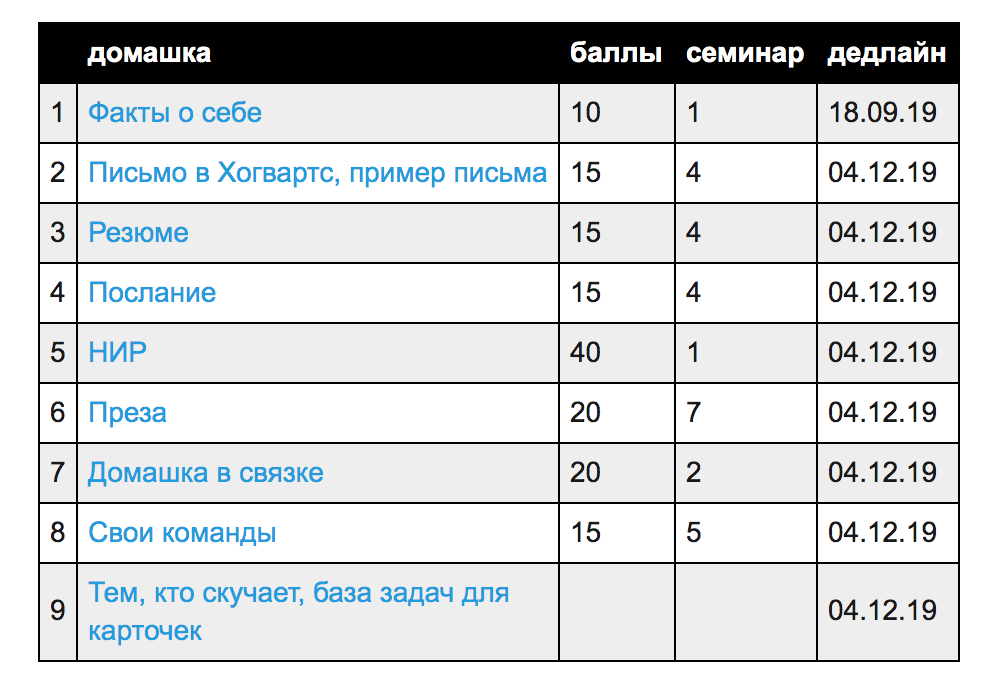
\includegraphics[scale=0.22]{hw.png}
	\end{column}
\end{columns}
\end{frame}


\begin{frame}{Первая домашка}
\begin{columns}
\begin{column}{.48\linewidth}
	\begin{itemize}
		\item  Первая домашка с ранним дедлайном
		\item  Нужно написать 10 правдивых фактов о себе
		\item  Описать 5 своих любимых формул и одну ненавистную
		\item  Вставить свою фотку и любимый мем
		\item  Составить таблицу своих любимых курсов на иканаме
	\end{itemize}
\end{column}	

	\begin{column}{.48\linewidth}
		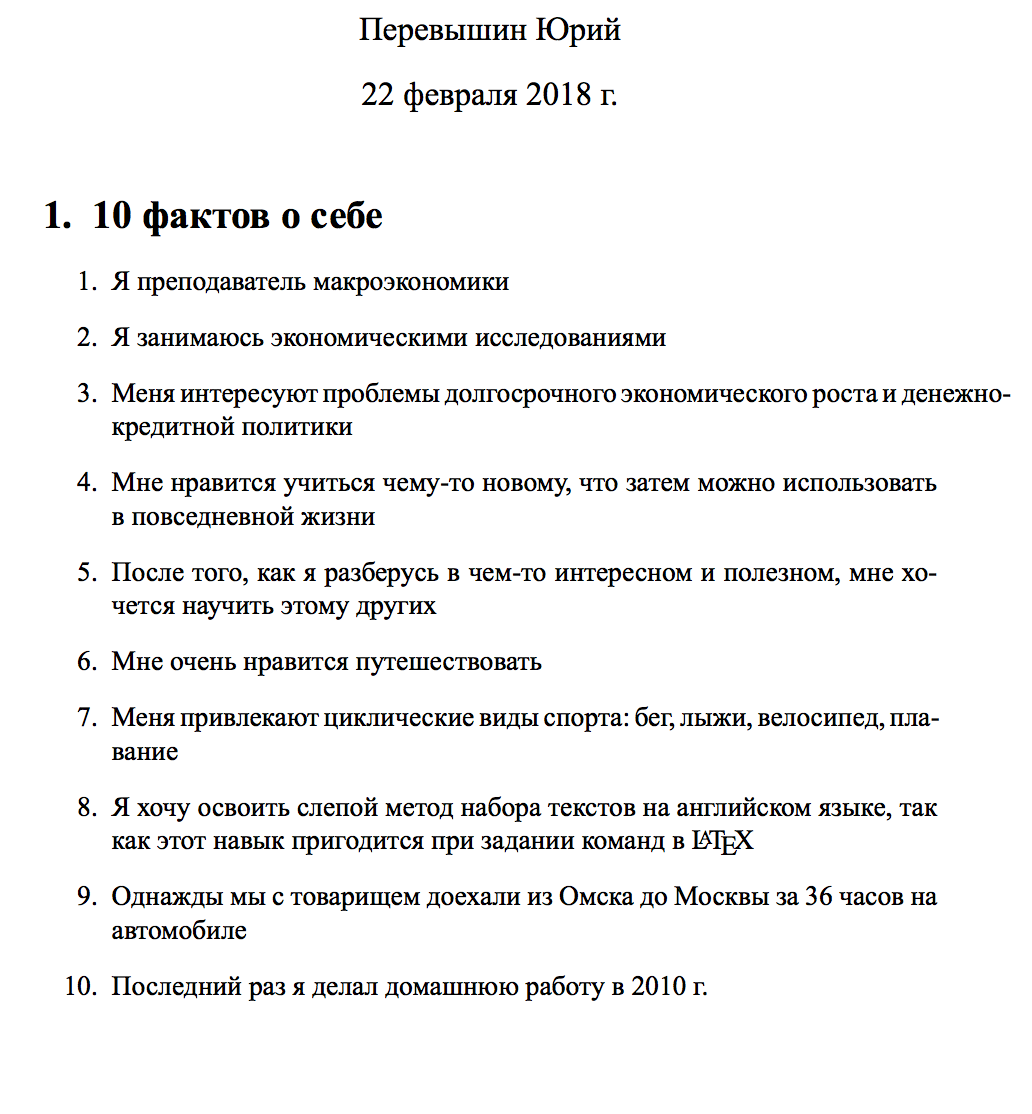
\includegraphics[scale=0.18]{hw_per.png}
	\end{column}
\end{columns}
\end{frame}



\begin{frame}
\frametitle{Куда идти за мудростью}

У нашего курса есть страничка на Github! Многие из вас уже были там и видели, что там много разной мудрости.
\vspace{1cm}

\begin{block}{Страничка курса:}
\vspace{3mm}
\centerline {\url{https://fulyankin.github.io/LaTeX/}}
\vspace{3mm}
\end{block}
\end{frame}



\section{Что за \LaTeX{} такой}


\begin{frame}
\frametitle{Что это вообще такое ?}
\alert{TeX} —  это созданная американским математиком и программистом Дональдом Кнутом система для верстки текстов с формулами.

\centering 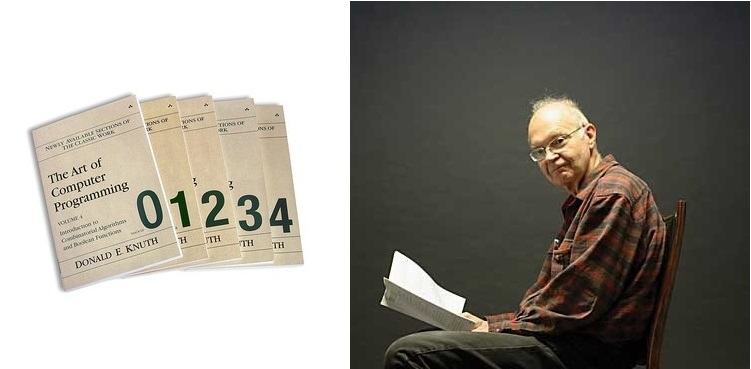
\includegraphics[scale=0.5]{knut.jpg}\\
\end{frame}


\begin{frame}
\frametitle{Откуда появился \LaTeX{}?}
\begin{columns}
	\begin{column}{.48\linewidth}
		\centering 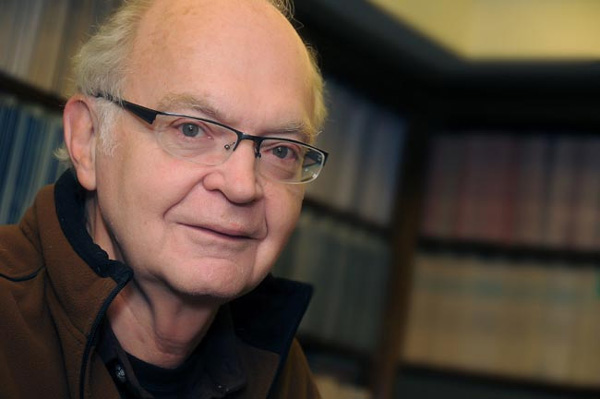
\includegraphics[scale=0.2]{DK.jpg}\\
		\mbox{ } \\
		Дональд Кнут создал в 1978 году программу \TeX.
	\end{column}
	
	\begin{column}{.48\linewidth}
		\centering Лесли Лэмпорт создал в 1984 году макропакет \LaTeX. \\
		\mbox{ } \\
		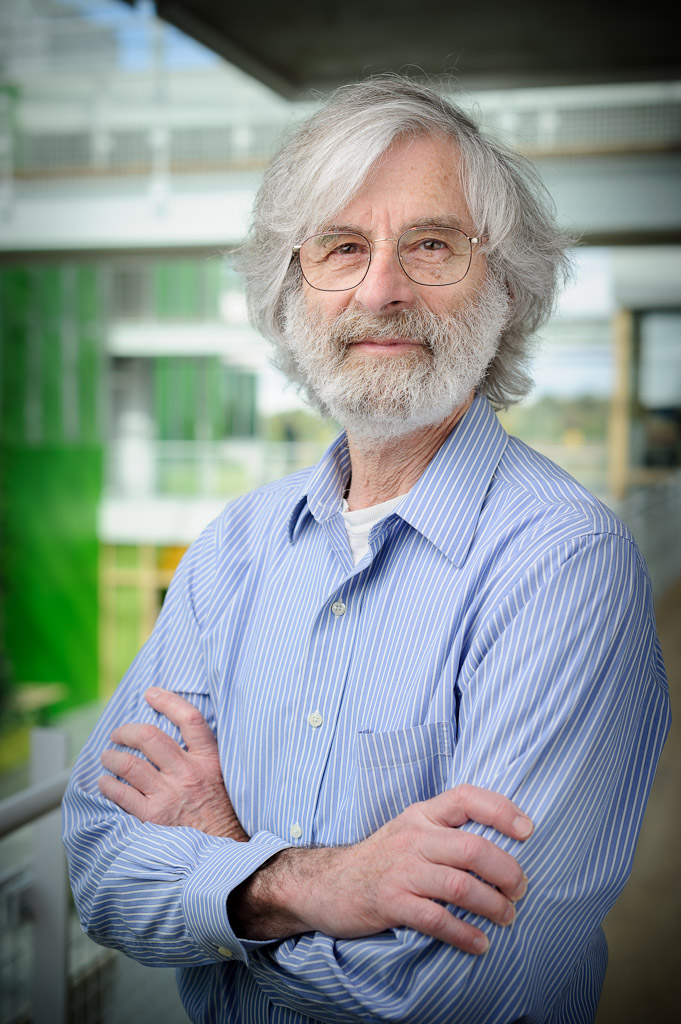
\includegraphics[scale=0.4]{LL.jpg}
	\end{column}
\end{columns}
\end{frame}


\begin{frame}{Движки}
\centering
\begin{tabulary}{\textwidth}{JcJ}
	\toprule
	движок			& рождение & отличие	\\[0.25em]
	\midrule
	\TeX{}				    & 1978 & начало пути  \\[0.25em]
	\LaTeX{}				& 1984 & расширение, упрощение \\[0.25em]
	\midrule
	
	pdf\LaTeX{}				& 2000 & сборка не dvi, а сразу pdf  \\[0.25em]
	Xe\LaTeX{}				& 2004 & юникод, куча шрифтов   \\[0.25em]
	Lua\LaTeX{} 		    & 2007 & язык Lua + Xe\LaTeX     \\[0.25em]
	\midrule
	bib\TeX{}				& 1985 &  удобная библиография  \\[0.25em]
	bib\LaTeX{} (biber)		& 2010 &  юникод, ряд улучшений    \\[0.25em]
	\bottomrule
\end{tabulary}

\href{https://habrahabr.ru/post/114610/}{Статья про движки на хабре}
\end{frame}


\begin{frame}
\frametitle{Почему \LaTeX{}?}
\begin{itemize}
\item Он позволяет делать красивые документы
\item Особенно документы с формулами
\item Большое и активное комьюнити, у которого всегда можно попросить о помощи
\item Он уютный!
\item Многие вещи, связанные с оформлением автоматизированы, что позволяет думать о содержании
\item Огромное количество различных пакетов и расширений в свободном доступе
\end{itemize}
\end{frame}


\begin{frame}{У \LaTeX{} хорошие друзья}
\centering

\includegraphics[width=0.9\linewidth]{ltx_friends.png}
\end{frame}



\section{Как работает \LaTeX}

\begin{frame}
\frametitle{\LaTeX{}  WYSIWYM}
\LaTeX{} не WYSIWYG (What You See Is What You GET).
\textbf{В WYSIWYG системах что автор видит на экране, то и получается на печати.}

\mbox{ }

\LaTeX{} WYSIWYM (What You See Is What You \alert{MEAN}).
\textbf{\LaTeX{} сам позаботится об оформлении, вам остаётся только думать о содержании!}
\end{frame}



\begin{frame}[fragile]
\frametitle{Как это работает}
Вы пишите свой текст с различными \alert{командами}, описывающими структуру текста, а \LaTeX{} преобразует их в красиво отформатированный pdf-документ!

\begin{mdframed}[backgroundcolor=LTXLightGreen]
В Португалии \verb|\textbf|\{дождь\} является \verb|\textit|\{причиной\}  не  работать.
\end{mdframed}

\centering
   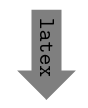
\includegraphics[scale=0.3]{fuc.png}%}

\begin{mdframed}[backgroundcolor=LTXLightGreen]
В Португалии \textbf{дождь} является \textit{причиной} не работать.
\end{mdframed}
\end{frame}


\begin{frame}[fragile]
\frametitle{Ещё примеры работы \LaTeX{}}

\begin{tabular}{p{7cm}p{4cm}}
\vspace{10mm} \verb|
\includegraphics[scale=0.15]{doge.png}| &  \begin{center} 
\includegraphics[scale=0.2]{doge.png} \end{center}
\end{tabular}
\vspace{3mm}
\begin{tabular}{p{7cm}p{4cm}}
\centering \verb|$\alpha^{x+5} + \sigma_{t}$| & \centering  $\alpha^{x+5}+\sigma_{t}$
\end{tabular}
\end{frame}


\begin{frame}[fragile]
\frametitle{Любой документ состоит из двух частей}
\begin{center}

\includegraphics[scale=0.28]{preamble.png} 
\end{center}
\end{frame}


\begin{frame}[fragile]
\frametitle{Необходимый минимум}
\begin{itemize}
	\item Каждый документ состоит из преамбулы и основной части
	\item \alert{Не надо каждый раз писать преамбулу с нуля!}
	\item Каждая команда начинается с \verb|\|
	\item Каждый документ начинается с \verb|\documentclass|
	\item В фигурных скобках \verb|{ }| указываются обязательные опции 
	\item В квадратных скобках \verb|[ ]| указываются необязательные опции
	\item Свои комментарии, которые \LaTeX{ } не видит, оставляются за \verb|%|
	\item Для английского языка этого достаточно, для русского нужно подключить кириллицу
\end{itemize}
\end{frame}


\begin{frame}[fragile]
\frametitle{Подключаем русский язык}
\begin{center}
	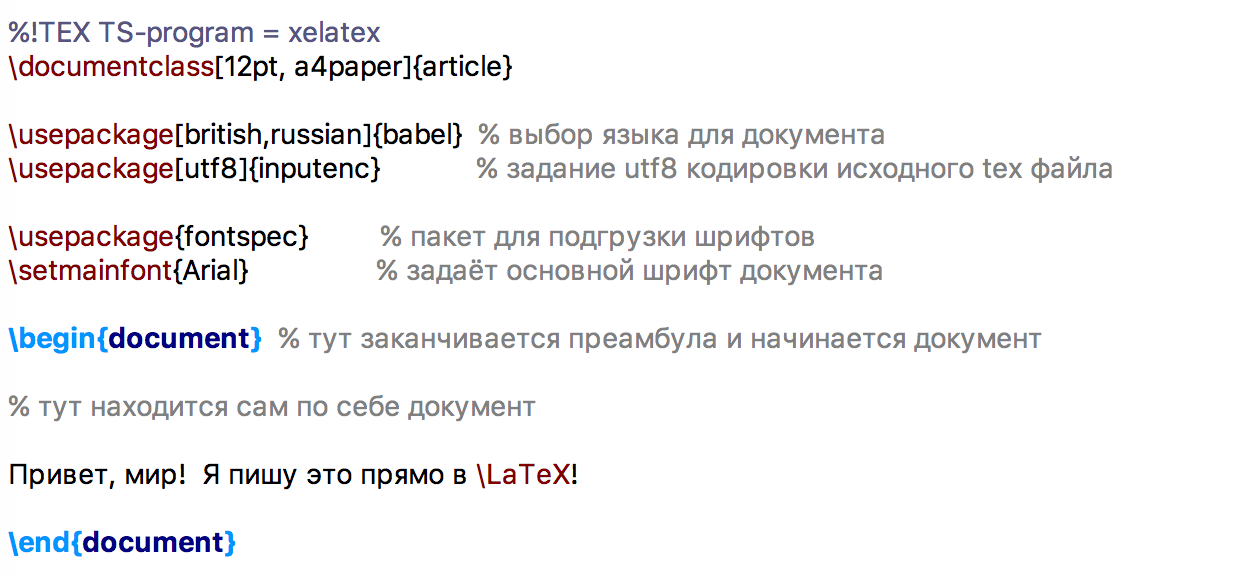
\includegraphics[scale=0.28]{preamble2.png} 
\end{center}
\end{frame}


\begin{frame}{Откуда берутся пакеты?}
\begin{columns}
\begin{column}{.66\linewidth}
\begin{itemize}
\item Их находят в капусте (нет)
\item Их скачивают с сайта \url{http://www.ctan.org}
\end{itemize}
\end{column}
\begin{column}{.33\linewidth}
\hfill 
\includegraphics[width=0.6\linewidth]{cabage.png}
\end{column}
\end{columns}
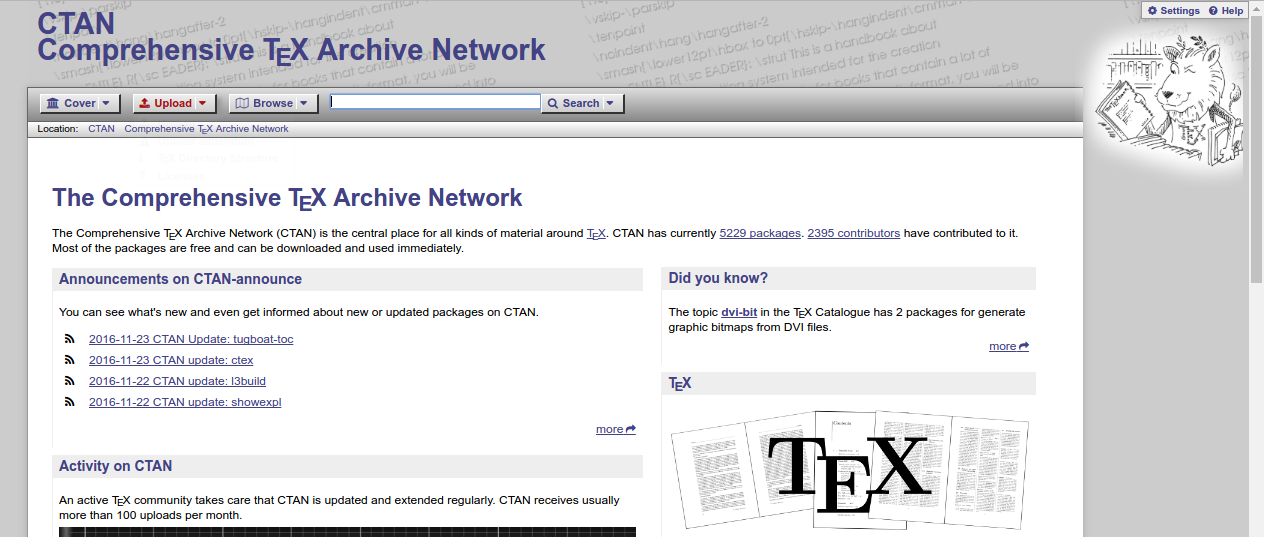
\includegraphics[width=0.6\linewidth]{CTAN.png}
\end{frame}


\begin{frame}[fragile]
\frametitle{Ещё пакеты}
\begin{center}
	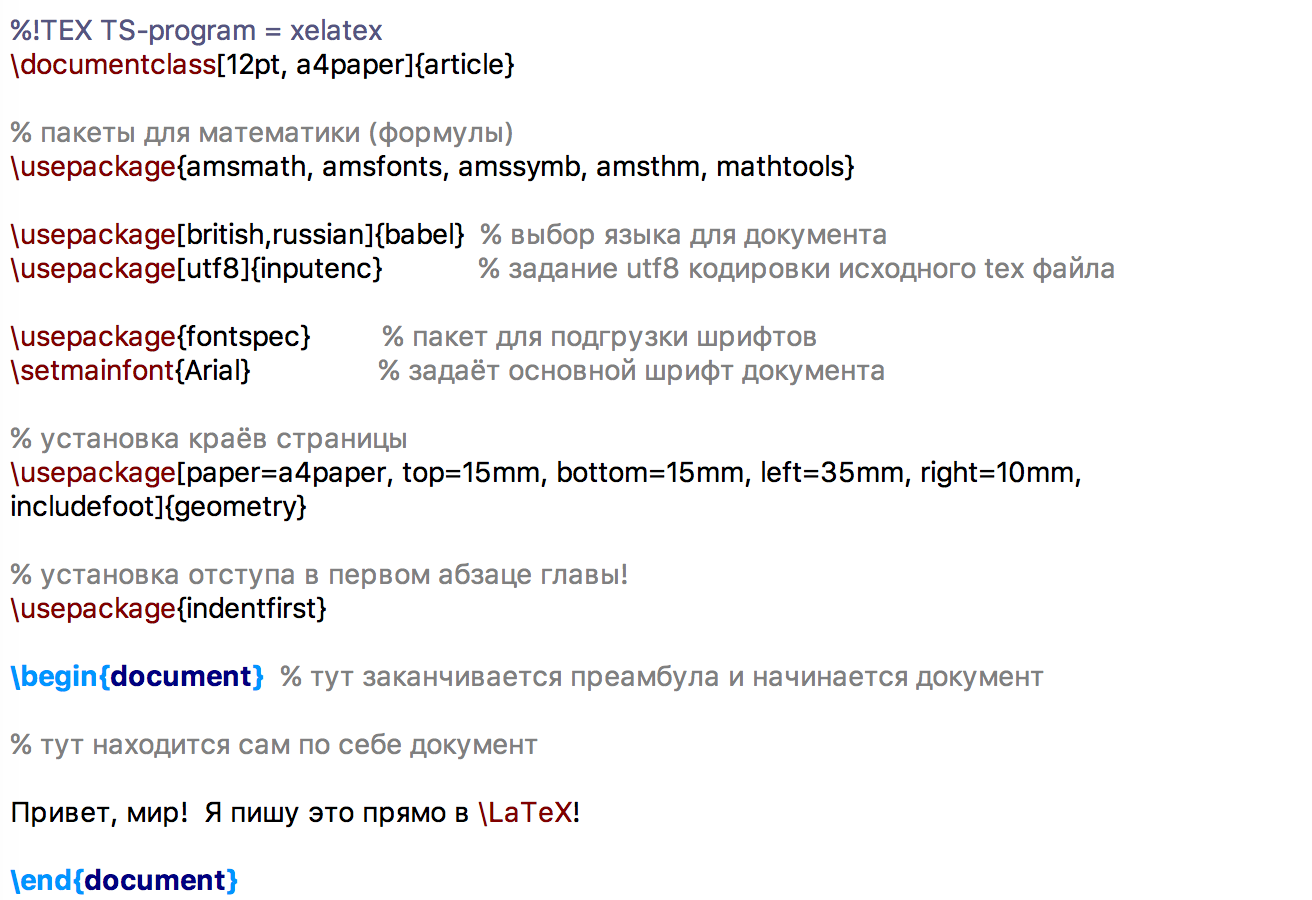
\includegraphics[scale=0.27]{preamble3.png} 
\end{center}
\end{frame}


\begin{frame}[fragile]
\frametitle{Набор текста}
    Между \verb|\begin{document}| и \verb|\end{document}|  находится ваш документ 
\begin{center}
	
\includegraphics[scale=0.28]{document1.png} 
\end{center}
\end{frame}


\begin{frame}[fragile]
\frametitle{Структура документа}
\begin{itemize}
	\item Чтобы структурировать документ на разделы просто используйте \verb|\section| и \verb|\subsection|
	\item Можно использовать \verb|\section*| и \verb|\subsection*|. А в чём, кстати, разница?  \pause
	\item Заголовки не будут нумероваться. На самом деле \verb|*| универсальный отключатель нумерации в \LaTeX{} 
\end{itemize}
\end{frame}

{
	\usebackgroundtemplate{ 
		\hspace{1.2cm}	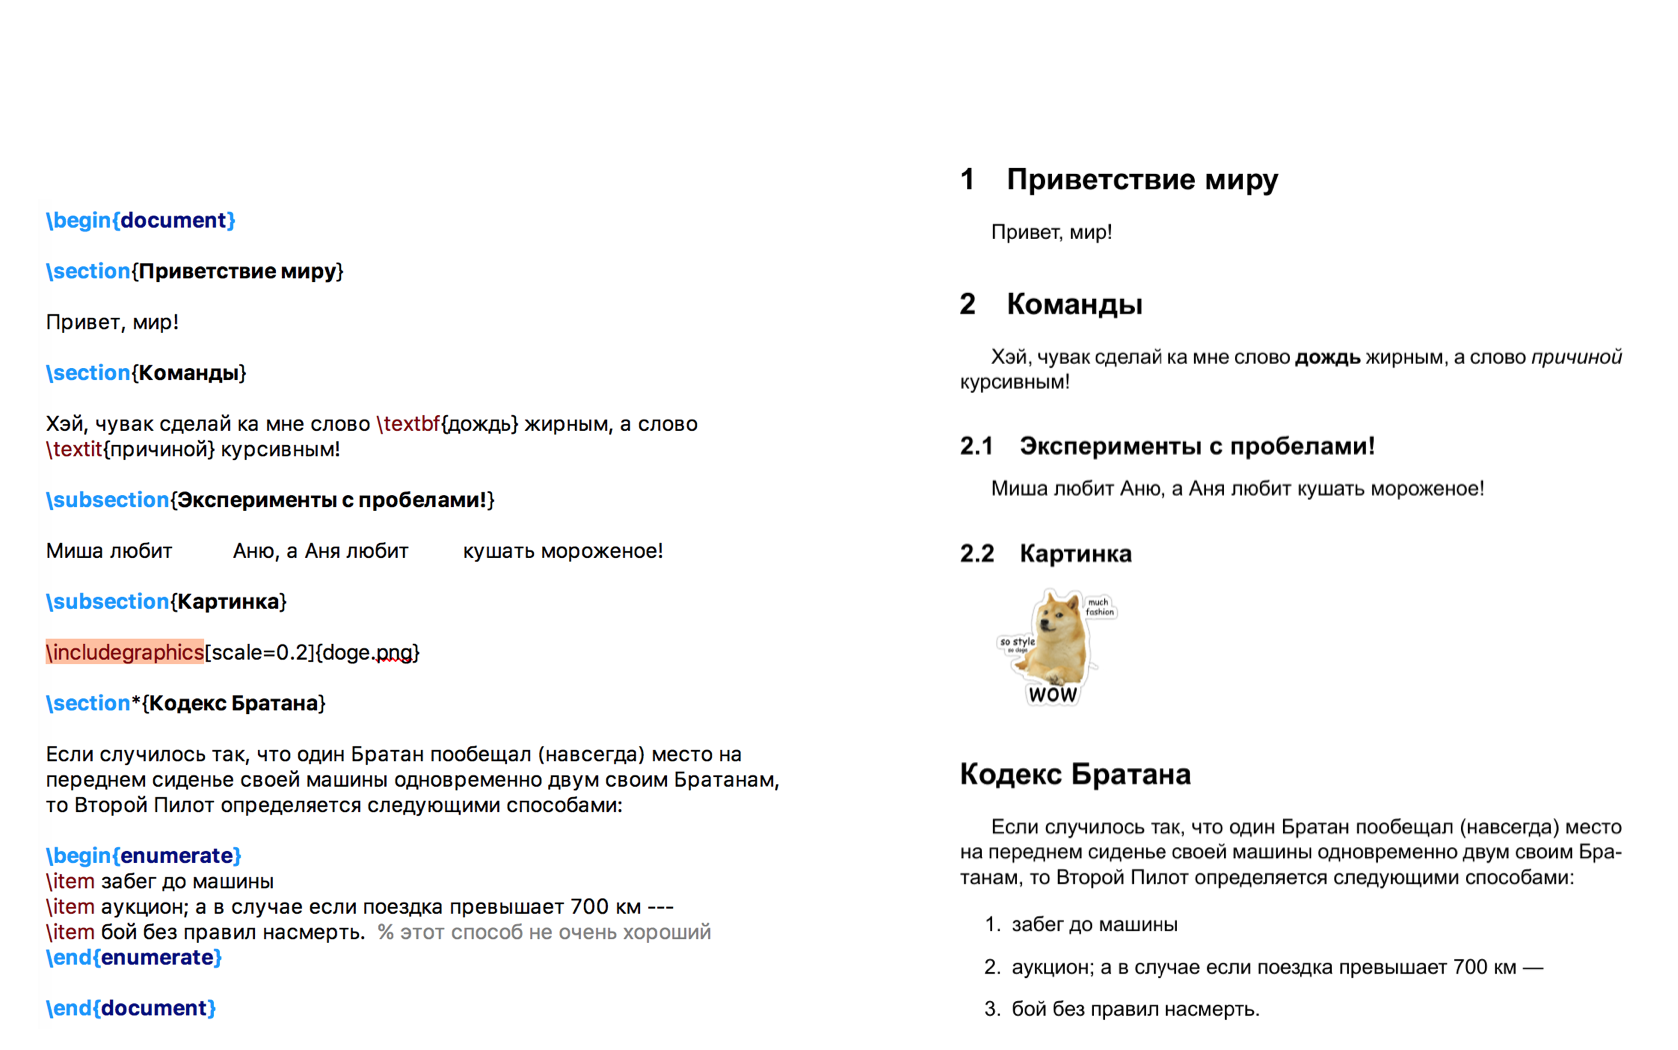
\includegraphics[width=1\linewidth]{document3.png}
	}
	\begin{frame}
\end{frame}
}


\begin{frame}[fragile]
\frametitle{Математический режим}

\begin{itemize}
	\item Cимвол \$ позволяет перейти в математический режим внутри текста. Один \$ открывает его, второй закрывает.
	\item С помощью символов \$\$ или \verb|\[| и \verb|\]| можно свесить формулу на отдельную строчку.
\end{itemize}
\begin{center}
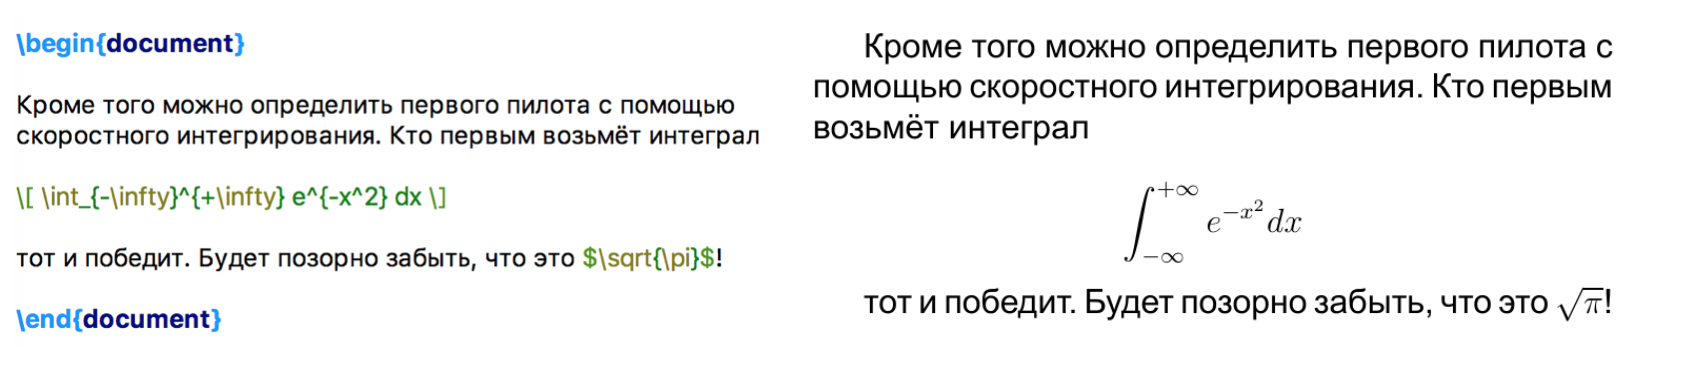
\includegraphics[scale=0.22]{document2.png} 
\end{center}
\end{frame}


\begin{frame}
\frametitle{Откуда взять формулу}
\begin{itemize}
	\item В \LaTeX{} можно найти символы на все случаи жизни $\Im$
	\item По {\color{blue} \href{http://detexify.kirelabs.org/classify.html}{этой ссылке}} расположен распознаватель символов!
	\item В книге Львовского есть огровное количество символов с подробными комментариями! Например:
\end{itemize}
\centering  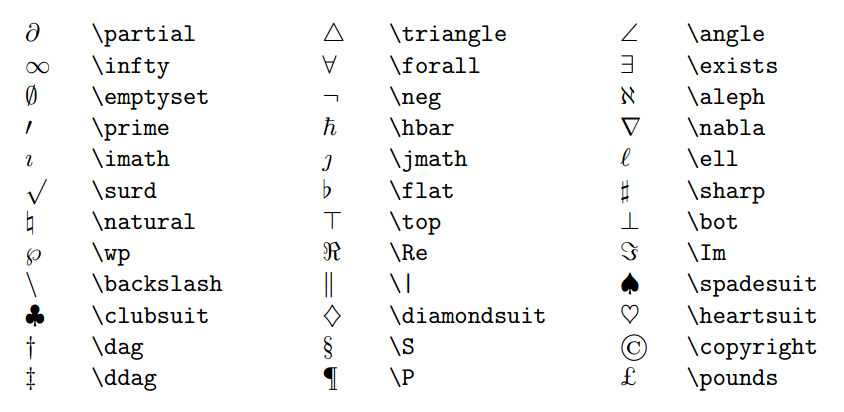
\includegraphics[scale=0.2]{table.png}
\end{frame}

\begin{frame}
\frametitle{Служебные символы}

\mbox{ }

\centering
\Large{ \$ \% \{ \} \# \& — служебные символы}

\mbox{ }

\begin{itemize}
	\item \normalsize{Чтобы использовать \$ или другой символ в тексте, надо написать $\setminus$\$.  Иначе будет выскакивать ошибка.}
\end{itemize}
\end{frame}

\section{Про картинки и таблицы} 

\begin{frame}{Векторные и растровые картинки} 
\begin{columns}
	\begin{column}{.55\linewidth}
		\begin{itemize}
			\item Растровые: PNG, GIF, JPEG \ldots
			\item Хранятся пиксельно, немасштабируются
			\item Веторные: PDF, EPS \ldots
			\item Хранятся описательно, масштабируются
			\item Сложный объект требует много места векторно и мало растрово.
		\end{itemize}
	\end{column}
	\begin{column}{.42\linewidth}
		
\includegraphics[width=0.99\linewidth]{rv.jpg}
	\end{column}
\end{columns}
\end{frame}

\begin{frame}[fragile]
\frametitle{Про картинки}
\begin{center}
	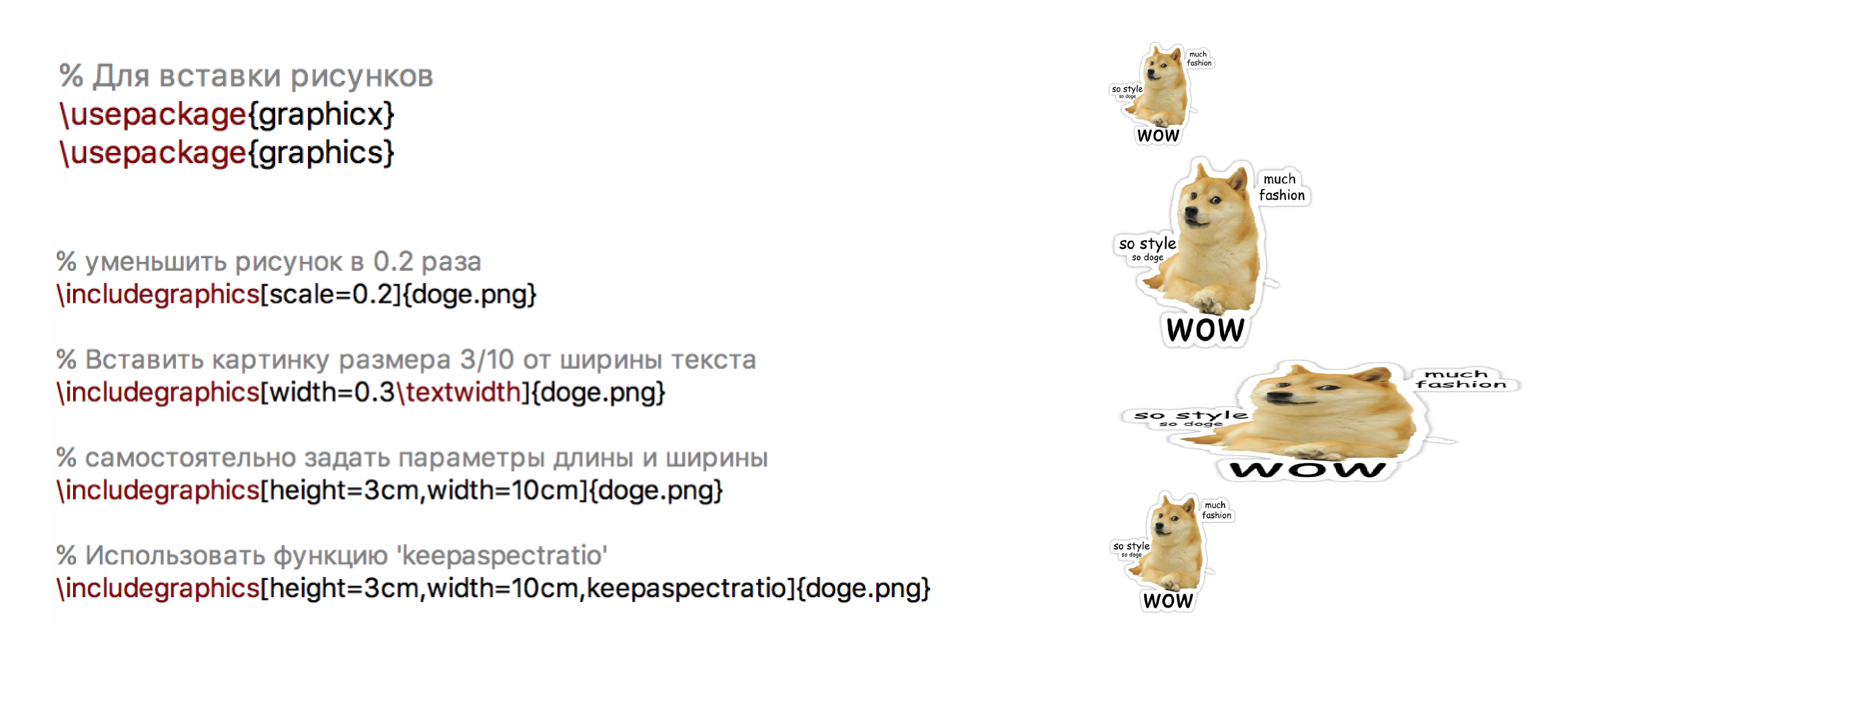
\includegraphics[scale=0.25]{document5.png} 
\end{center}
\end{frame}


\begin{frame}[fragile]{ }
\begin{block}{Единицы измерения в \LaTeX}
	\centering 
	\begin{tabulary}{\textwidth}{JccL}
		\toprule
		pt & & &пункт (0.35 mm) \\
		pc & & &пика  (12 pt)   \\
		mm & & &миллиметр       \\
		cm & & &сантиметр       \\
		in & & &дюйм            \\
		em & & &ширина буквы M используемого шрифта \\
		ex & & &высота буквы x используемого шрифта \\
		\bottomrule
	\end{tabulary}
\end{block}
\end{frame}


\begin{frame}[fragile]{ }
\begin{block}{И ещё немного длин в \LaTeX}
\centering 
\begin{tabulary}{\textwidth}{JccL}
	\toprule
	\verb|\pagewidth|  & & &ширина страницы \\
	\verb|\pageheight| & & &высота страницы \\
	\verb|\textwidth|  & & &ширина текста   \\
	\verb|\textheight| & & &высота текста   \\
	\verb|\linewidth|  & & & длина текста в текущем окружении \\
	\bottomrule
\end{tabulary}
\end{block}
\end{frame} 


\begin{frame}[fragile]
\frametitle{Про таблицы}

\begin{center}
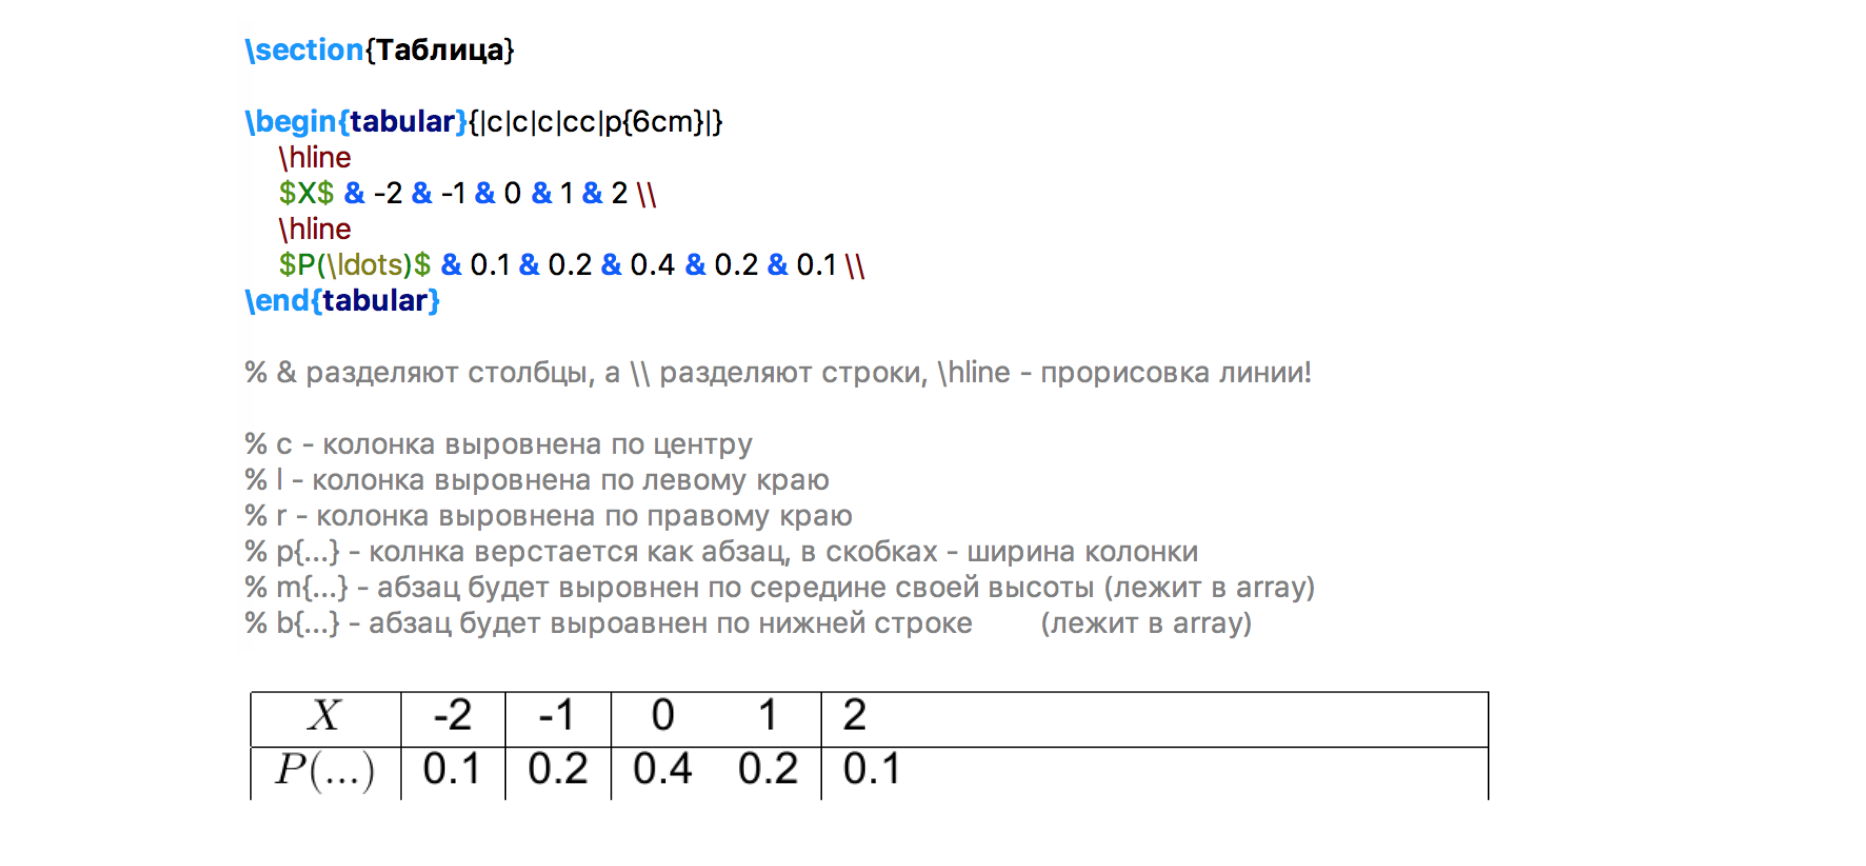
\includegraphics[scale=0.21]{document6.png} 
\end{center}
\end{frame}

\begin{frame}
\begin{block}{Типы колонок в таблицах}
	\centering 
	\begin{tabulary}{\textwidth}{JL}
		\toprule
		c & колонка выровнена по центру \\
		l & колонка выровнена по левому краю\\
		r & колонка выровнена по правому краю\\
		p\{ \} & колонка создаётся как абзац, в скобках ширина колонки \\
		\bottomrule
	\end{tabulary}
\end{block}

\alert{Не забывайте о существовании Quick Tabular \ldots}
\end{frame}
 

\begin{frame}{Про картинки и таблицы}
\begin{itemize}
\item Мы ещё не раз поговорим про картинки и таблицы.  Готовьтесь к этому :3 
\item Обратите внимание, что \alert{таблицы  —  это слабое место теха.} Их надо вбивать вручную, со всеми разделителями, чёрточками и это больно. Но есть автоматические способы рисовать их. Есть даже способы перегонять их из R. Но об этом рассказ будет в следущей серии. 
\end{itemize}
\end{frame}



\section{Создаём наш первый файл}

\begin{frame}{Можно работать на своём компьютере}
\begin{center}
	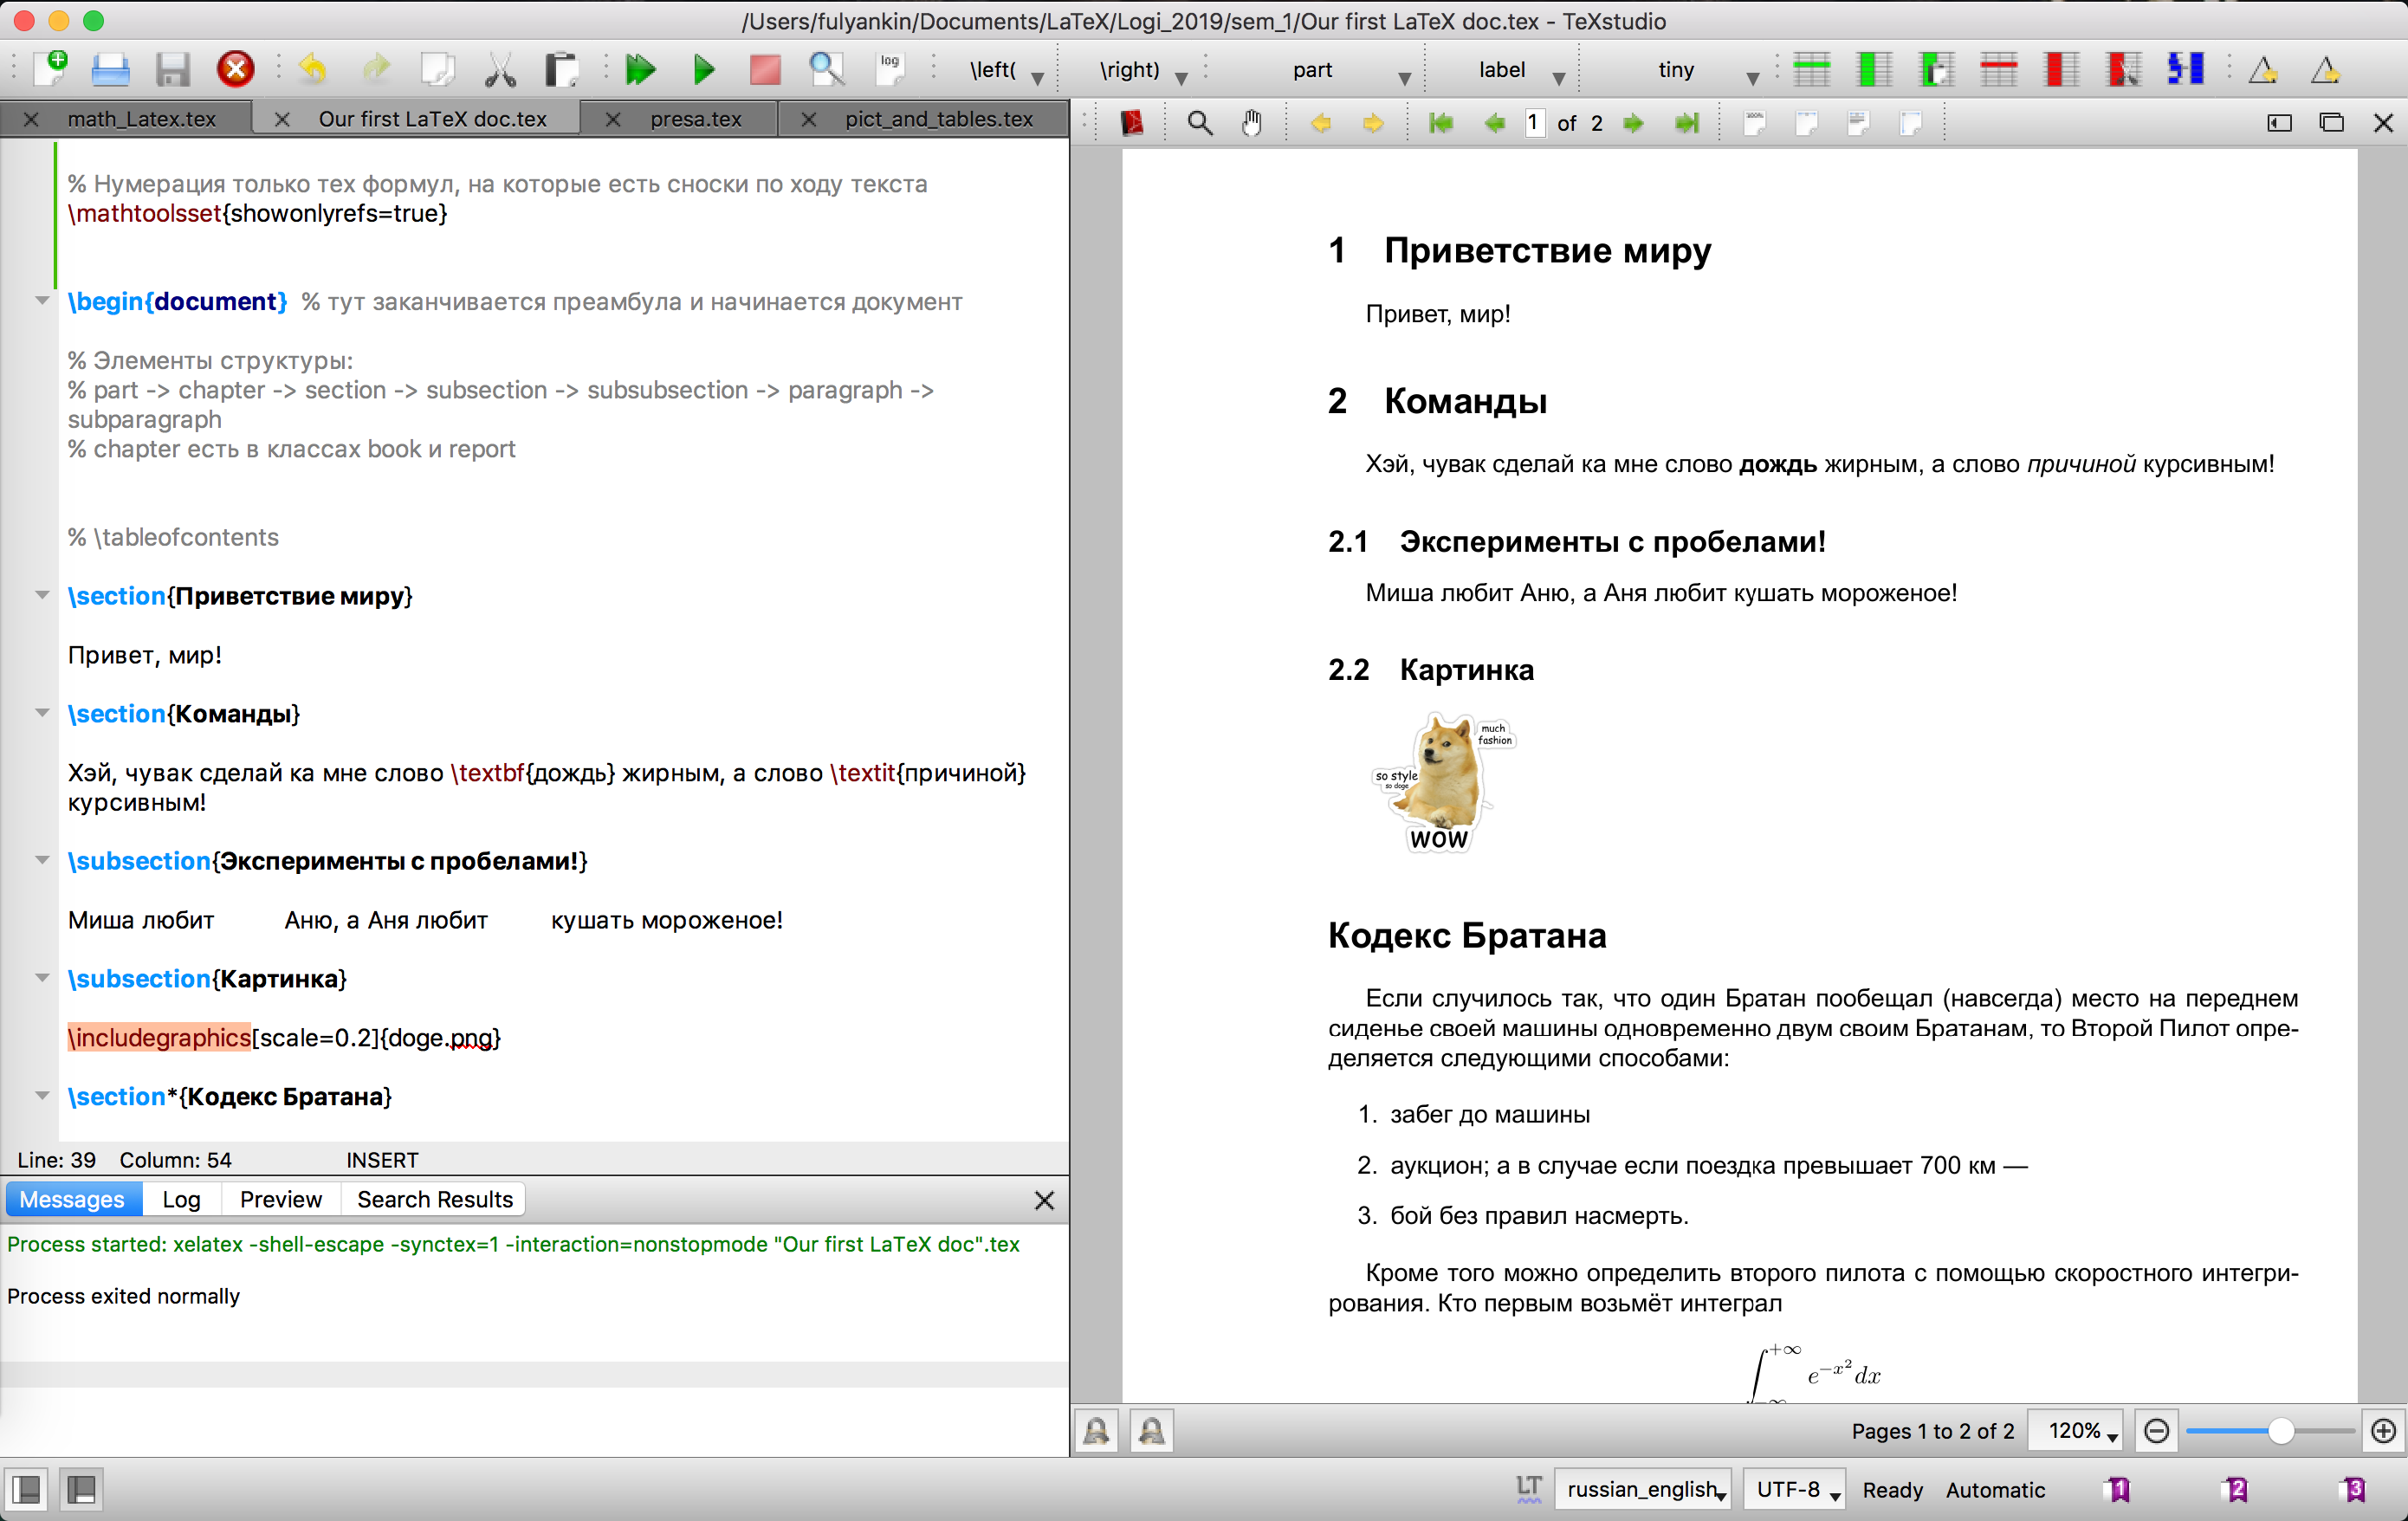
\includegraphics[scale=0.12]{work_comp.png} 
\end{center}
\end{frame}


\begin{frame}{Компиляция и её результаты}

\centering
	\begin{tabulary}{\linewidth}{JcJ}
		\toprule
		  файл	  & & предназначение \\[0.25em]
		\midrule
		  .tex    & & мы пишем в этом файле  \\[0.25em]
		  .pdf    & & наш документ  \\[0.25em]
		  .log    & & логи, информация обо всём, что произошло во время компиляции  \\[0.25em]
		  .aux    & & карта документа, в нём записаны все ссылки, номера страниц, табоиц и т.д.  \\[0.25em]
          .synctex     & & позволяет нажать в pdf правую кнопку и перейти к соответствующему месту в tex-файле  \\[0.25em]
		\bottomrule
	\end{tabulary}
\end{frame}


\begin{frame}{Можно работать в онлайне}
\begin{center}
	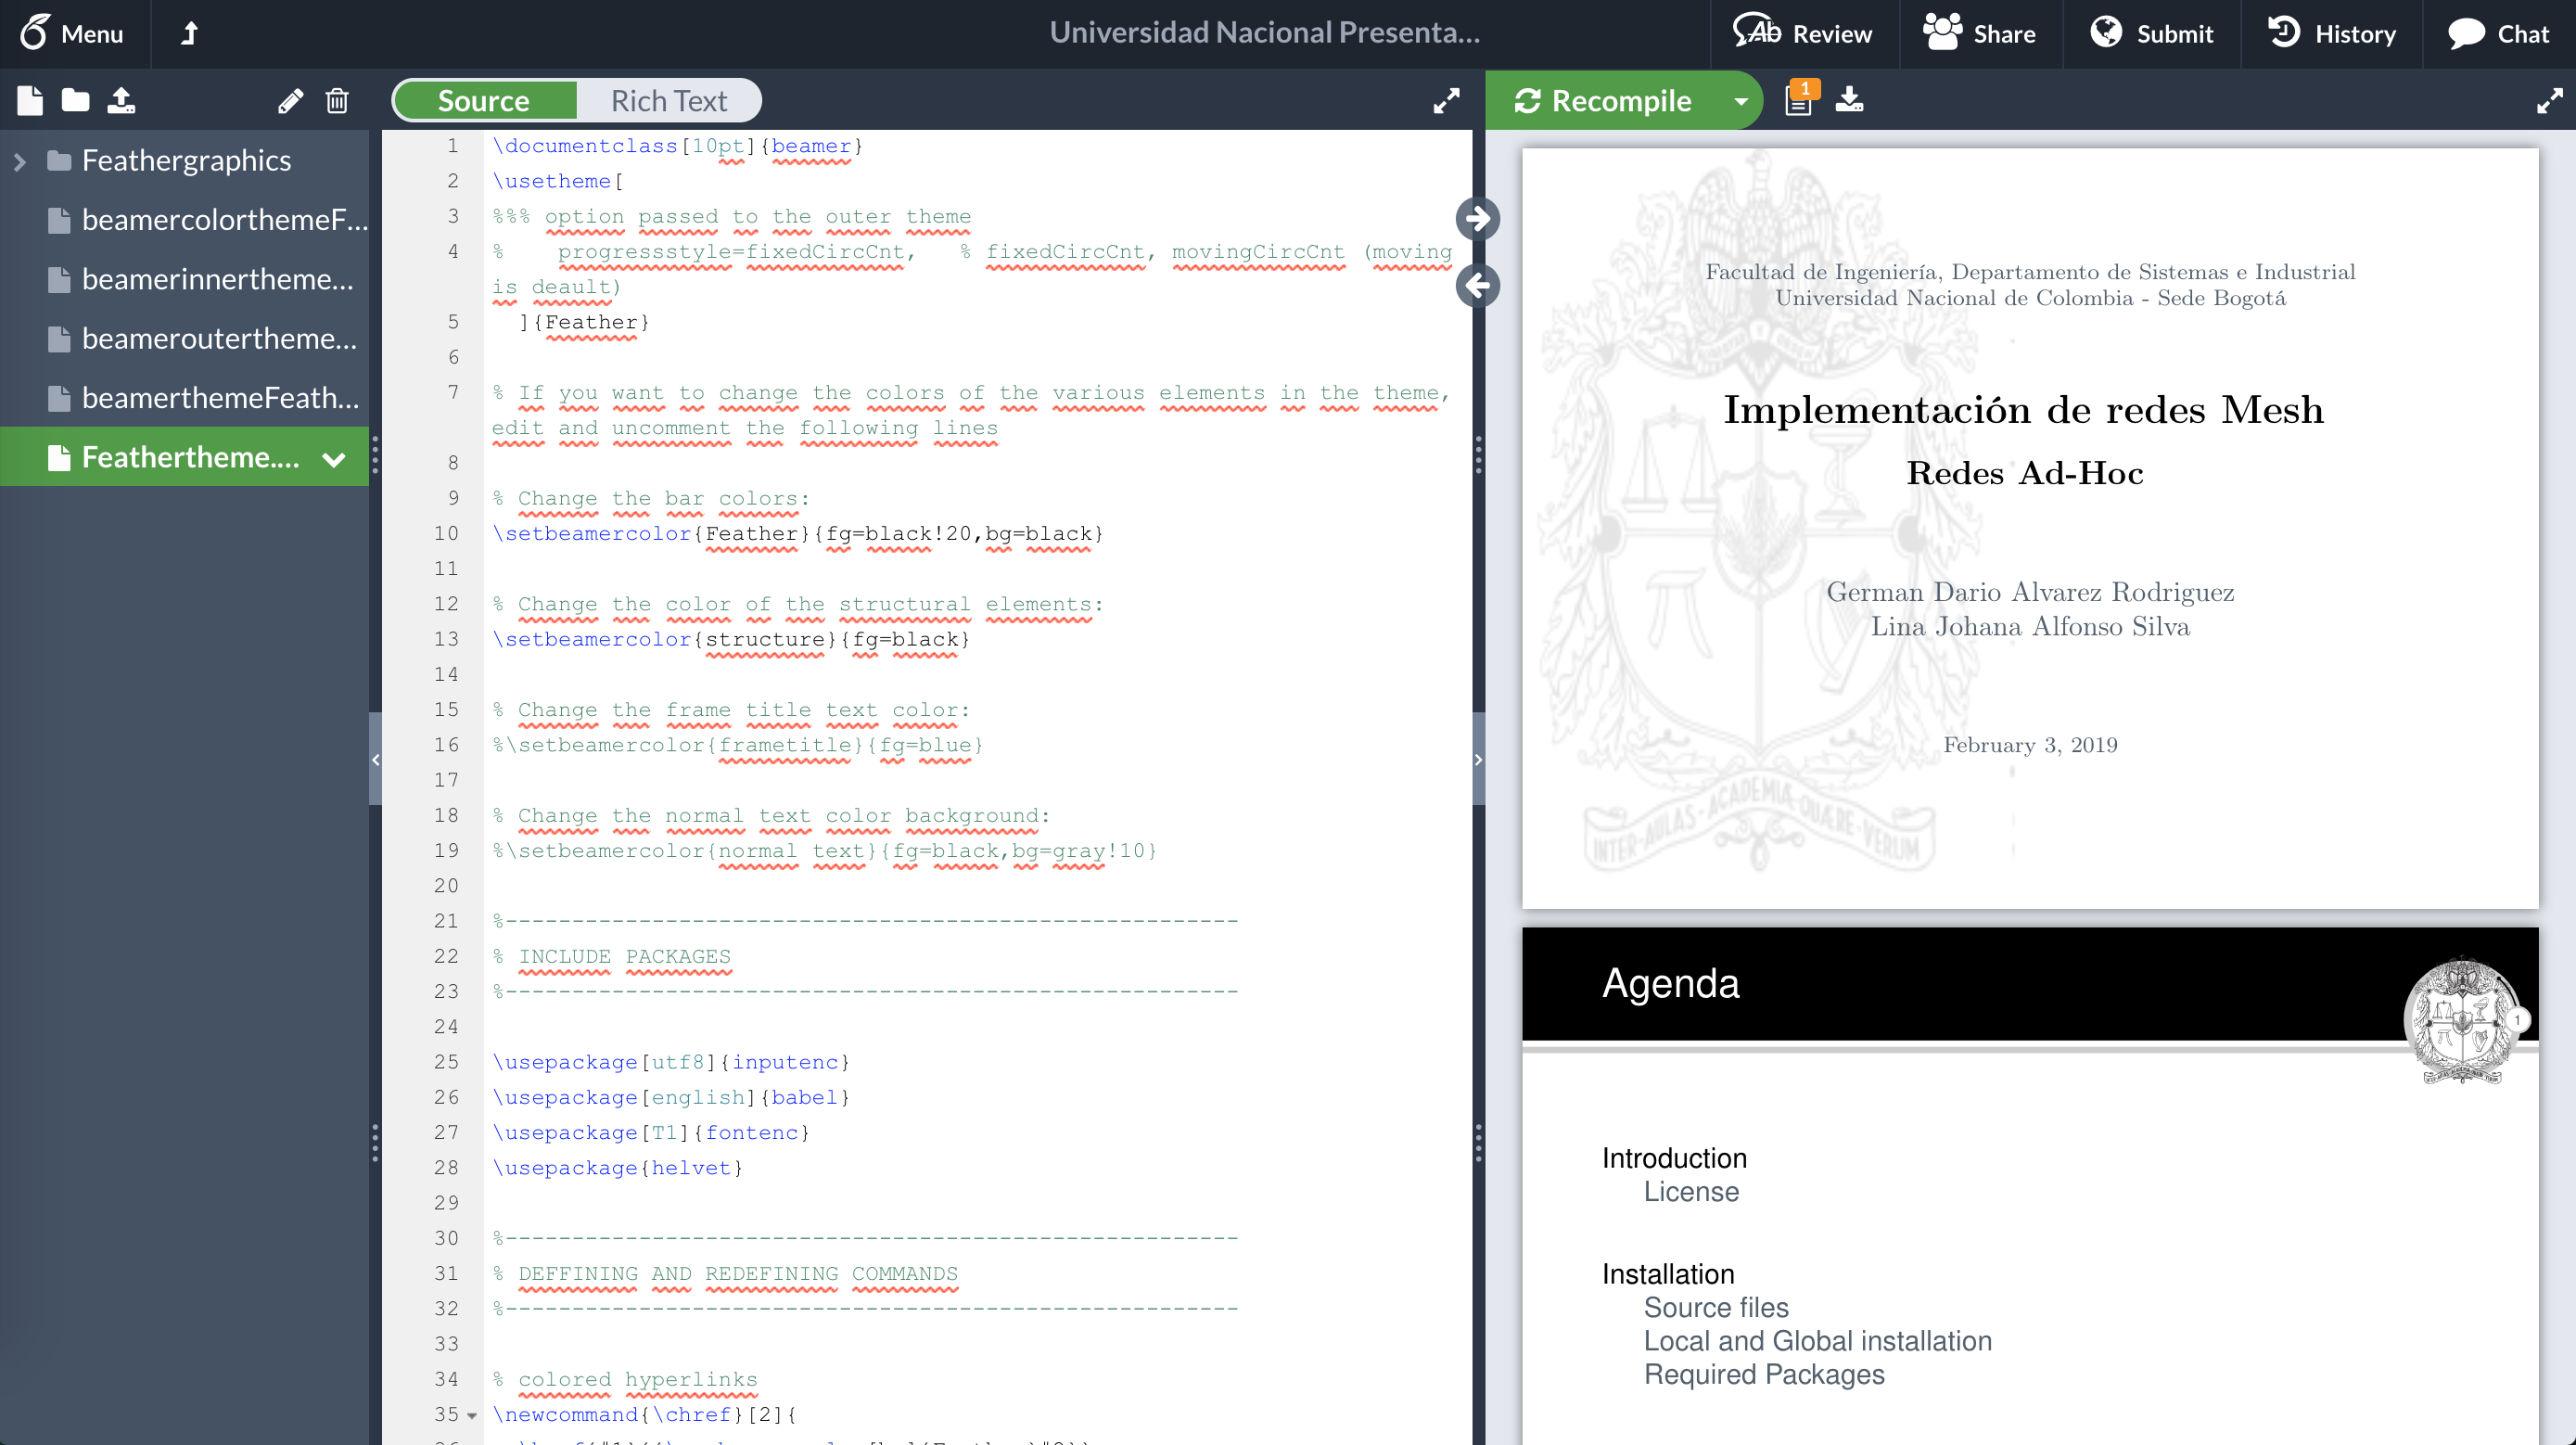
\includegraphics[scale=0.13]{online_work.png} 
\end{center}
\end{frame}


\begin{frame}{Можно работать в онлайне}

Наш первый документ, который мы собирали выше, можно найти по ссылке:

\vspace{1cm}

\begin{block}{Страничка курса:}
	\vspace{3mm}
	\centerline {\url{ Вставить сюда ссылку}}
	\vspace{3mm}
\end{block}
\end{frame}


\begin{frame}{Шаблоны}
\centering
\url{http://www.latextemplates.com/}


\includegraphics[width=0.4\linewidth]{template1.png}

\url{https://www.overleaf.com/latex/templates}

\includegraphics[width=\linewidth]{template2.png}
\end{frame}


\section{ТЕХ - ЗЛО! НАДО ПИСАТЬ КОД!} 

\begin{frame}
\Large
\begin{block}{\Large Вопрос года:}
	Как в Word сделать оглавление? 
\end{block}
\end{frame}


{
\usebackgroundtemplate{ 
	\hspace{1.2cm}	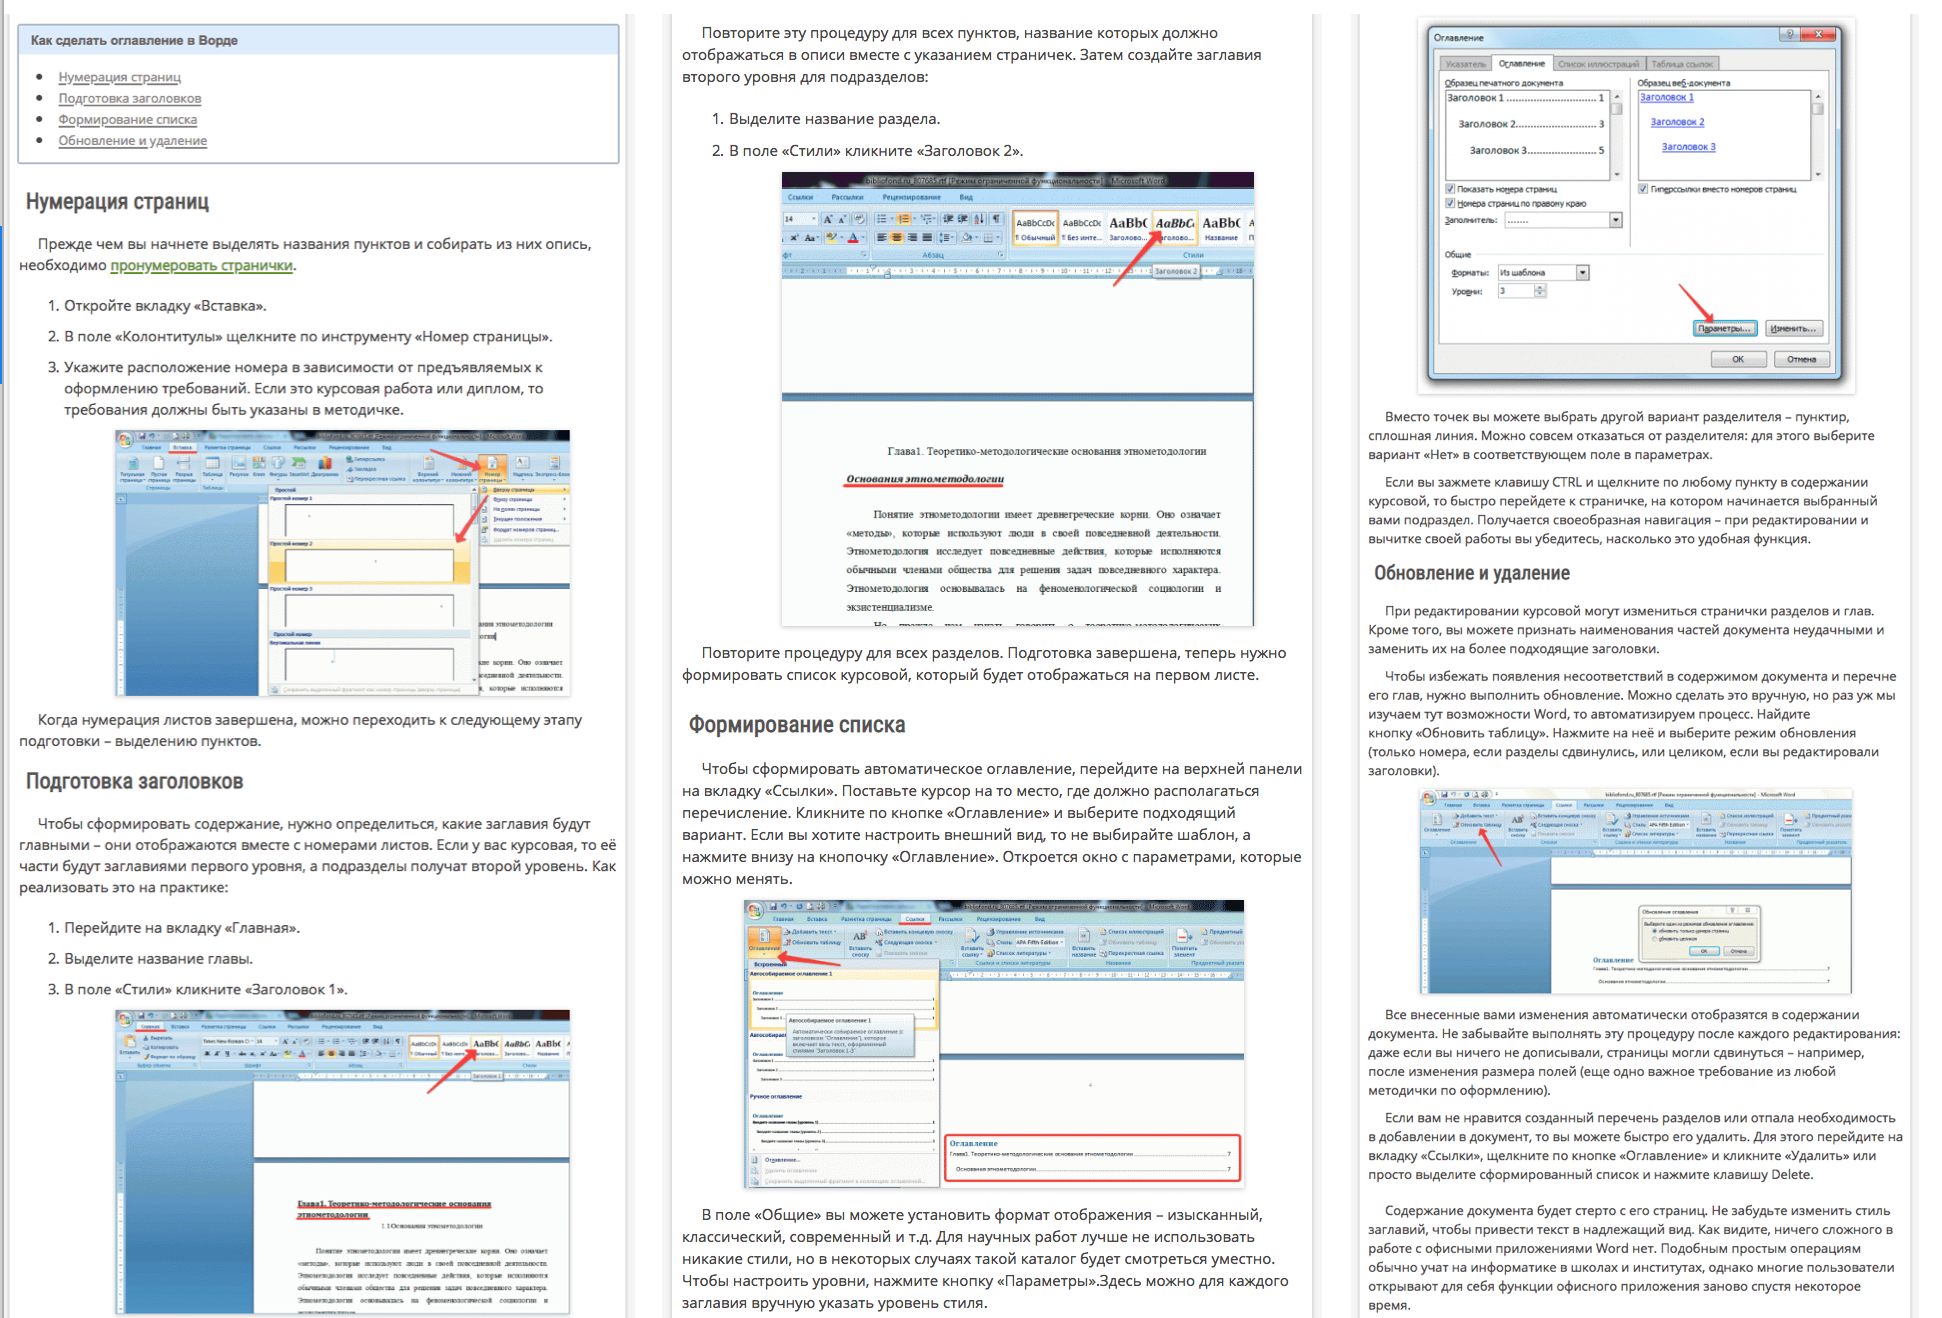
\includegraphics[width=0.98\linewidth]{word_tblofcont.png}
}
\begin{frame}
\end{frame}
}


\begin{frame}
\Large
\begin{block}{\Large Вопрос дня:}
Как в \LaTeX{ } сделать оглавление? 
\end{block}
\end{frame}


\begin{frame}
\mbox{ }

\centering
\Huge \alert{$\setminus$tableofcontent}

\mbox{ }
\end{frame}


\begin{frame}
\Large
\begin{block}{\Large Главный вопрос вселенной:}
А как узнать эту информацию? 
\end{block}
\pause 

\mbox{ }

\begin{block}{\Large Ответ:}
Загуглить!
\end{block}
\end{frame}


\begin{frame}[fragile]
\frametitle{Секрет сущего}
\begin{itemize}
\item Что в ворде, что в техе вам придётся гуглить возникающие у вас вопросы и как-то осваиваться в программе.
\item В техе вы загуглите один раз и навсегда добавите код в преамбулу, после тех всё сделает сам. 
\item В ворде вы будете гуглить каждый раз заново, и делать всё вручную. 
\end{itemize}
\end{frame}


\begin{frame}{How to \ldots  а также Error: \ldots}
\centering 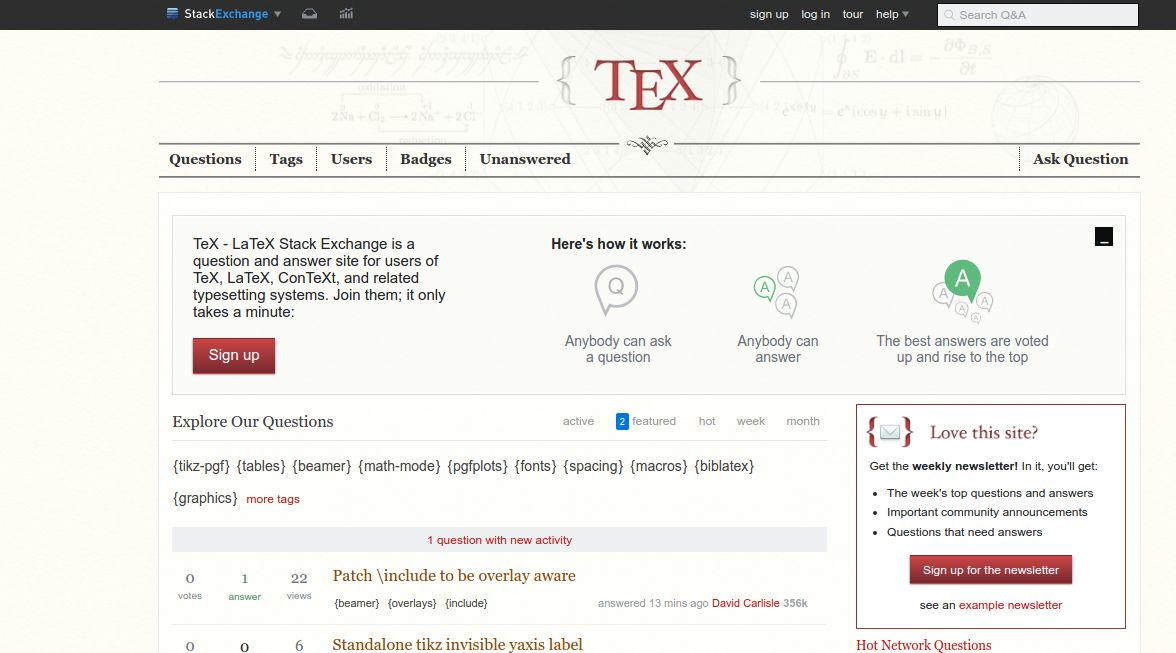
\includegraphics[width=0.8\linewidth]{texexchan.png}\\
\end{frame}


\begin{frame}{Мой рук}
\centering 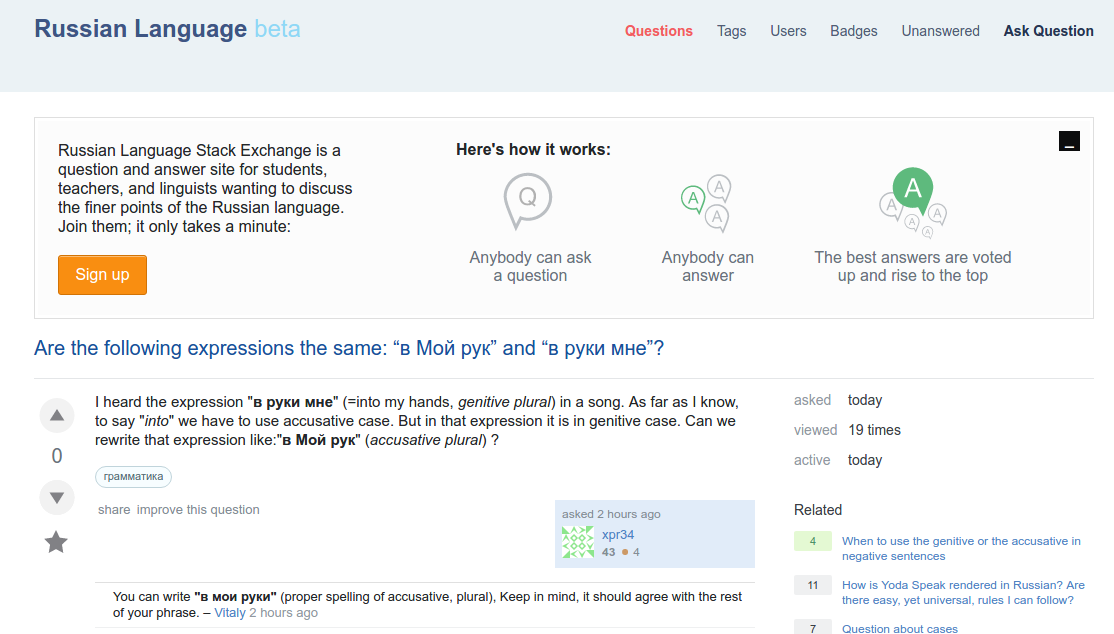
\includegraphics[width=0.8\linewidth]{russia.png}\\
\end{frame}


\begin{frame}{Мемы про Stack Overflow}
\begin{columns}
\begin{column}{.48\linewidth}
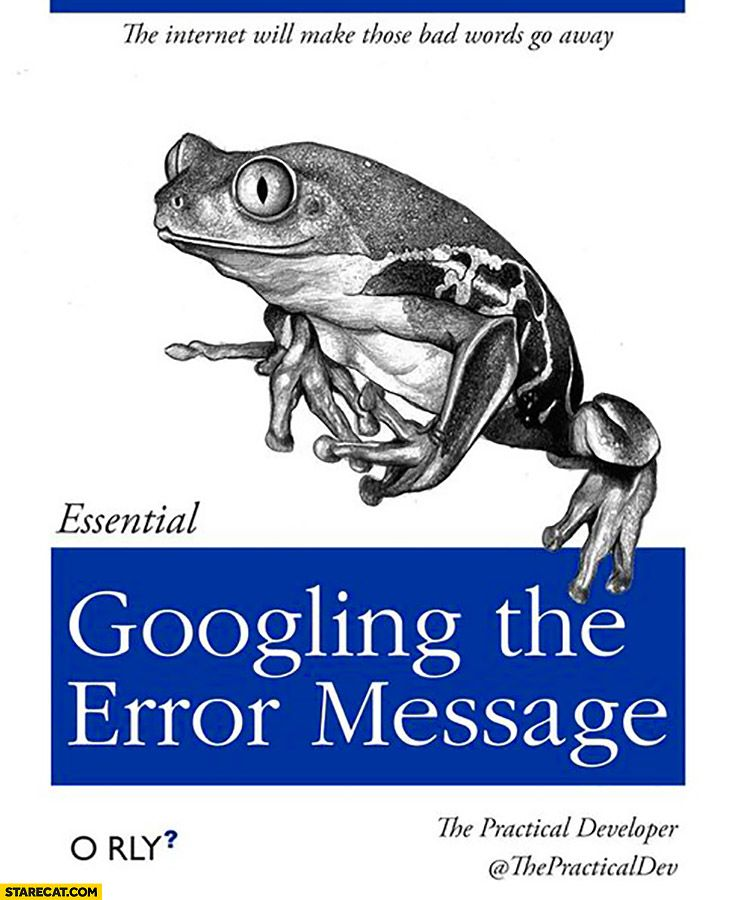
\includegraphics[width=0.8\linewidth]{googling.jpg}\\
\end{column}
\begin{column}{.48\linewidth}
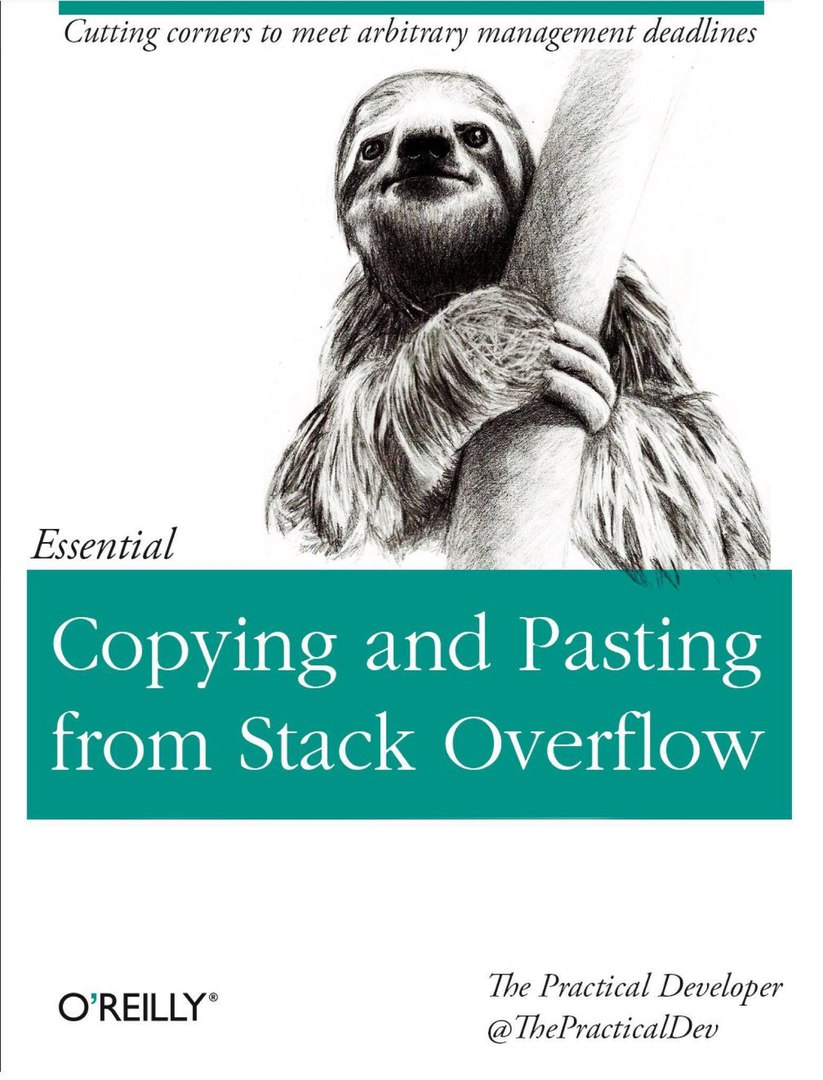
\includegraphics[width=0.8\linewidth]{copypast.jpg}\\
\end{column}
\end{columns}
\end{frame}




\section{Главная идея теха в трёх примерах}

\begin{frame}{Пример 1: формулы}
\Large
\begin{block}{\Large Что мы хотим:}
	\begin{itemize}
		\item Хотим вбить пару формул
		\item Хотим, чтобы они пронумеровались 
	\end{itemize}
\end{block}
\end{frame}


\begin{frame}{Пример 1: формулы}
\begin{center}
	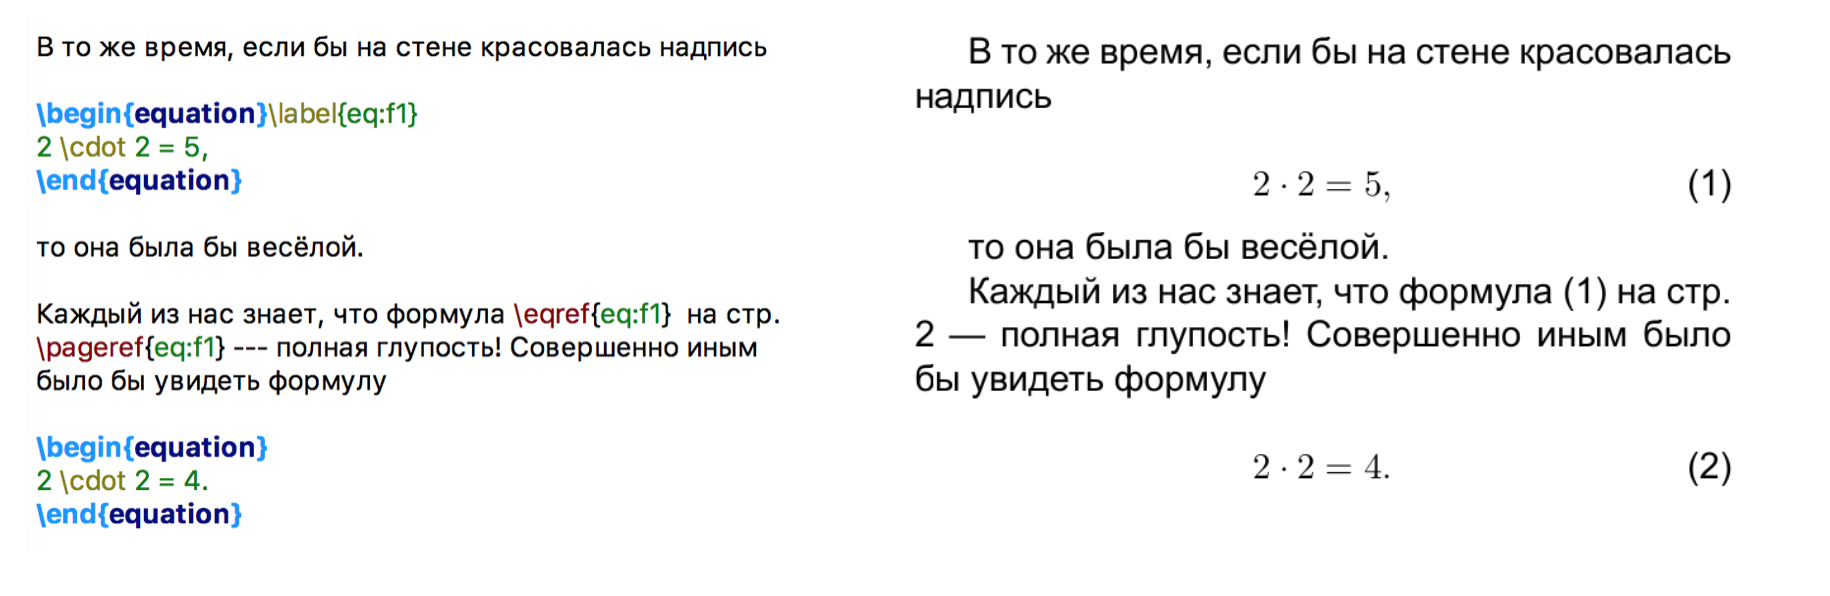
\includegraphics[scale=0.23]{ex1_1.png} 
\end{center}
\end{frame}


\begin{frame}{Пример 1: формулы}
\Large
\begin{block}{\Large Что мы хотим:}
	\begin{itemize}
		\item Неожиданно нам захотелось вставить ещё одну формулу в самое начало
	\end{itemize}
\end{block}
\end{frame}


\begin{frame}{Пример 1: формулы}
\begin{center}
	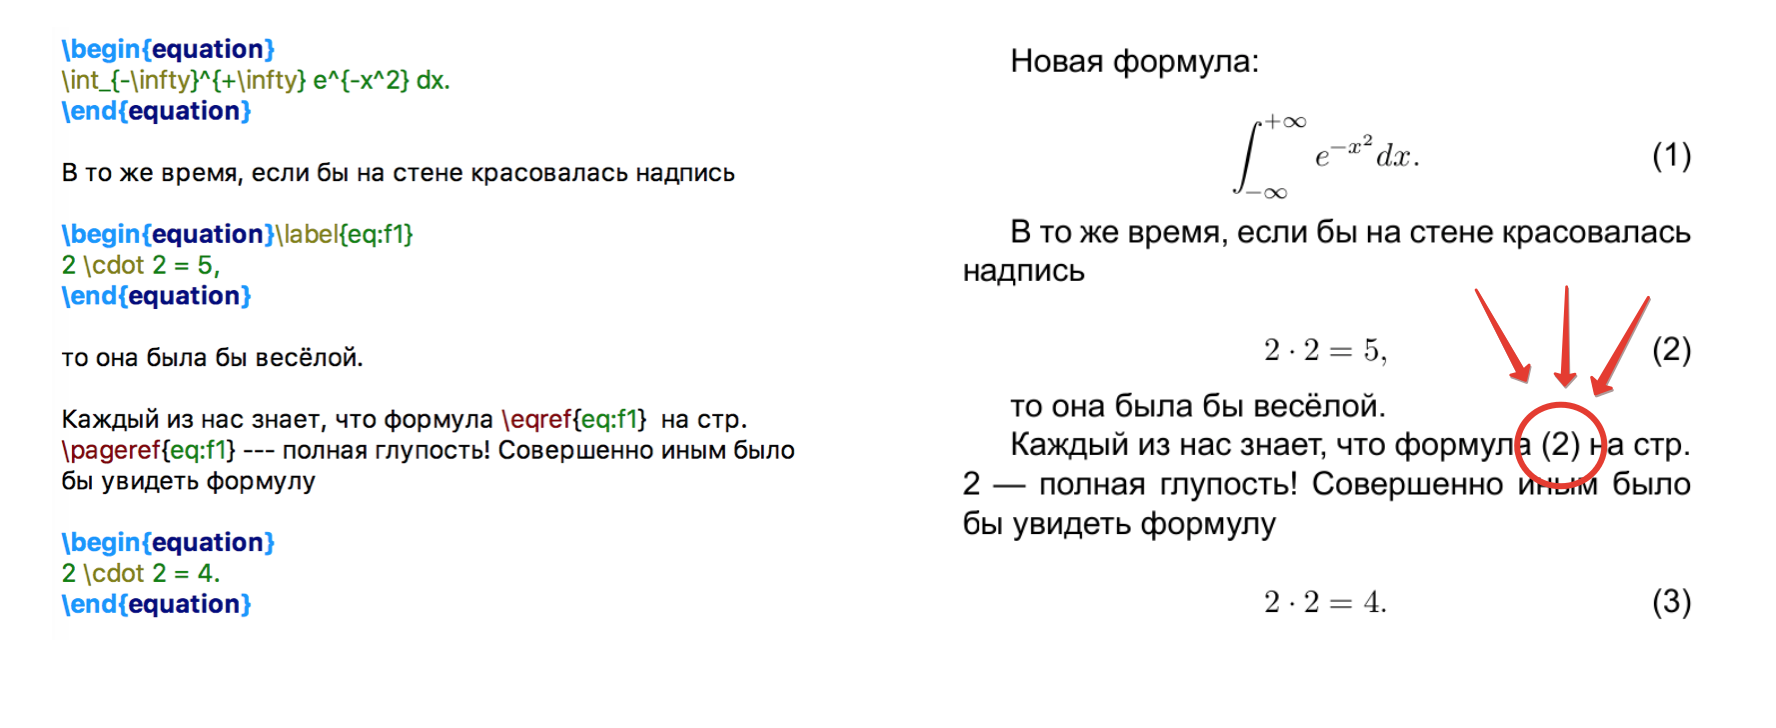
\includegraphics[scale=0.23]{ex1_2.png} 
\end{center}
\end{frame}


\begin{frame}{Пример 1: формулы}
\Large
\begin{block}{\Large Что мы хотим:}
	\begin{itemize}
		\item У нас не приняли диплом. Сказали, что пронумерованы должны быть только те формулы, на которые в тексте есть сноски.
	\end{itemize}
\end{block}
\end{frame}


\begin{frame}{Пример 1: формулы}
\begin{center}
	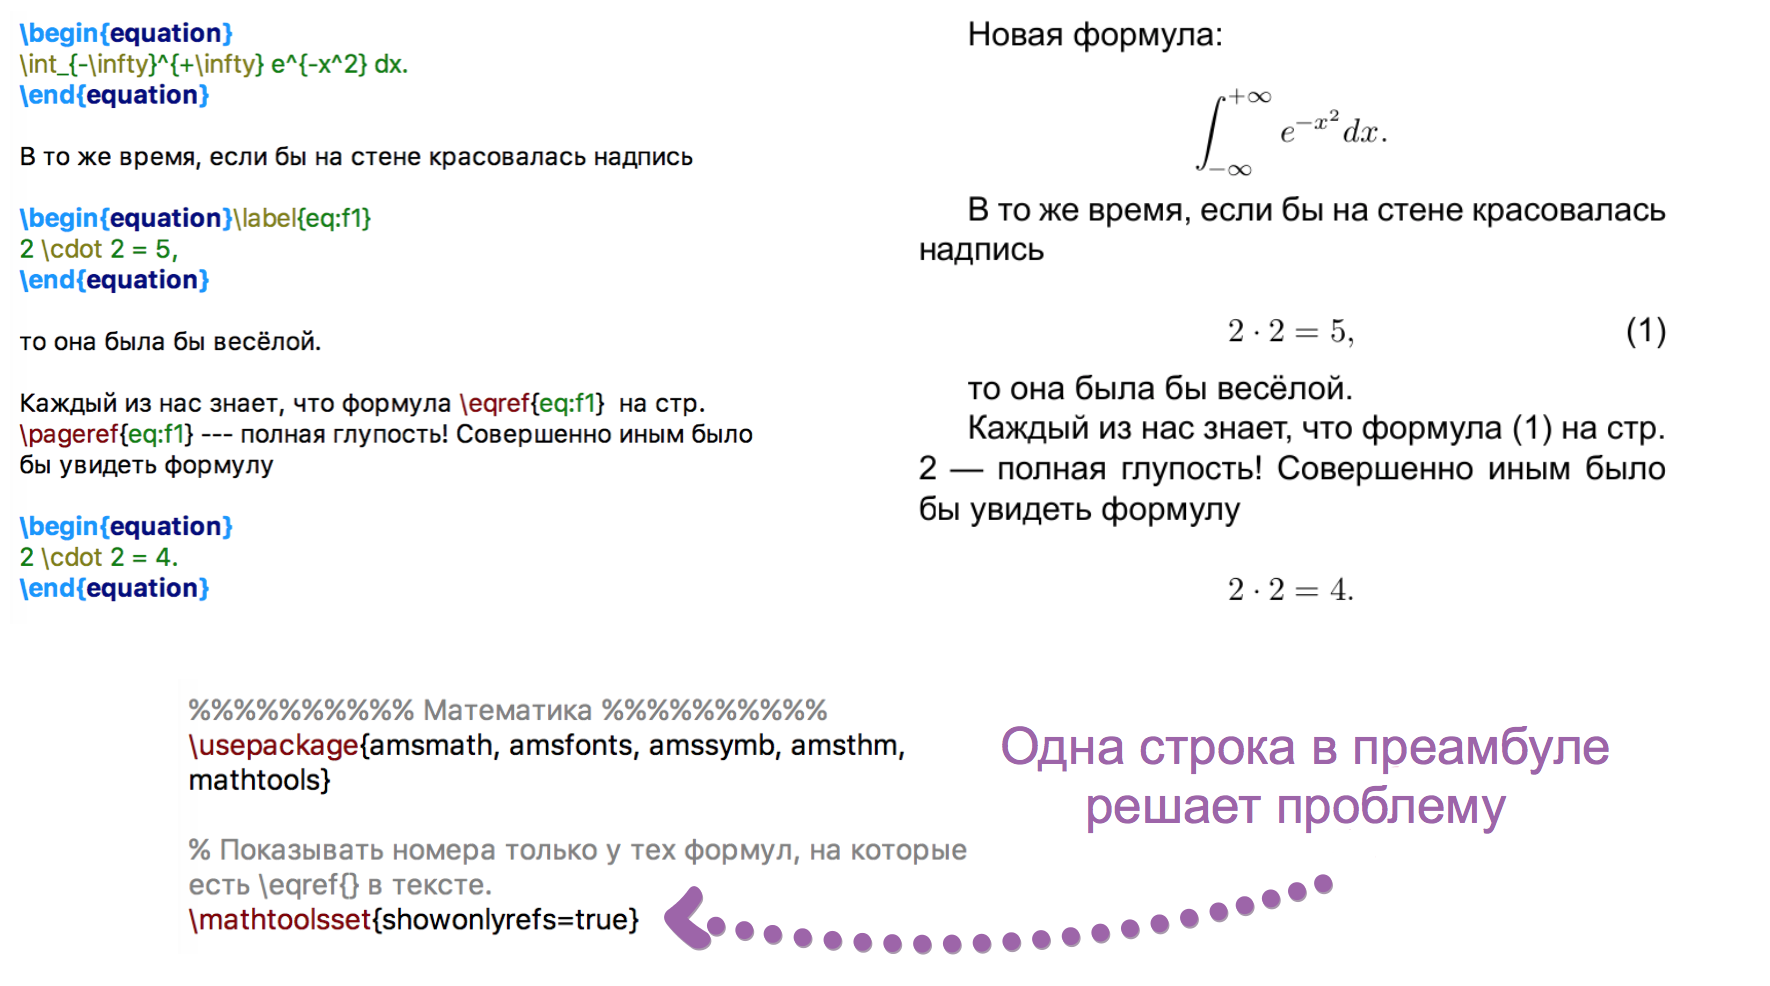
\includegraphics[scale=0.18]{ex1_3.png} 
\end{center}
\end{frame}


\begin{frame}{Пример 2: списки}
\Large
\begin{block}{\Large Что мы хотим:}
	\begin{itemize}
		\item Завести список годных сериалов
		\item Посмотреть их
	\end{itemize}
\end{block}
\end{frame}


\begin{frame}{Пример 2: списки}
\begin{center}
	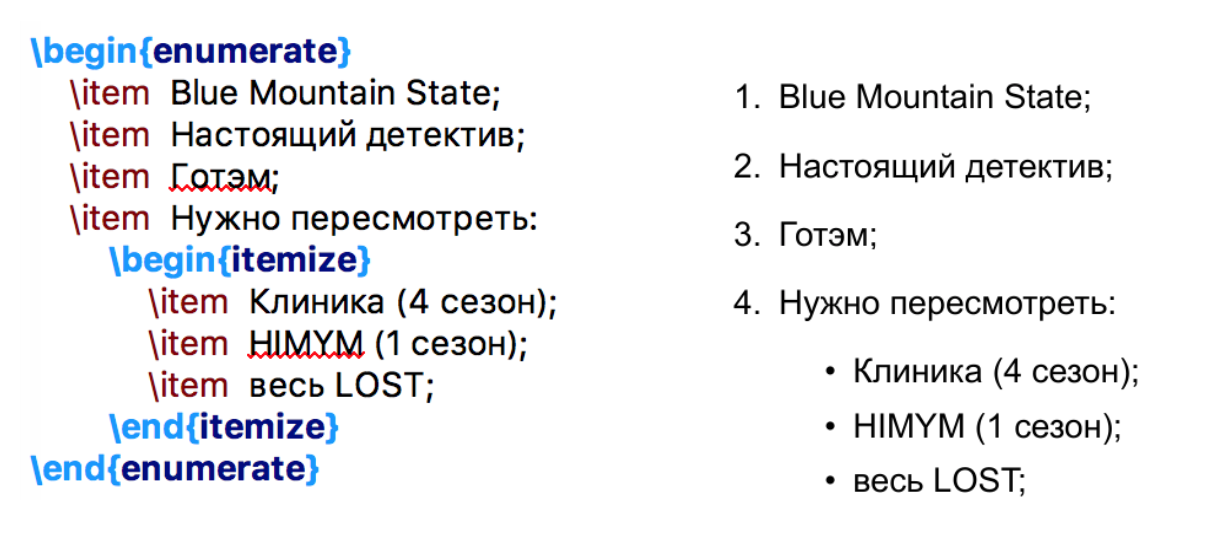
\includegraphics[scale=0.25]{ex2_1.png} 
\end{center}
\end{frame}


\begin{frame}{Пример 2: списки}
\Large
\begin{block}{\Large Что мы хотим:}
	\begin{itemize}
		\item Деканат не утвердил наш список 
		\item Они хотят, чтобы все сериалы были перечислены через буквы, а не цифры, а кружочки надо поменять на любой другой символ
	\end{itemize}
\end{block}
\end{frame}


\begin{frame}{Пример 2: списки}
\begin{center}
	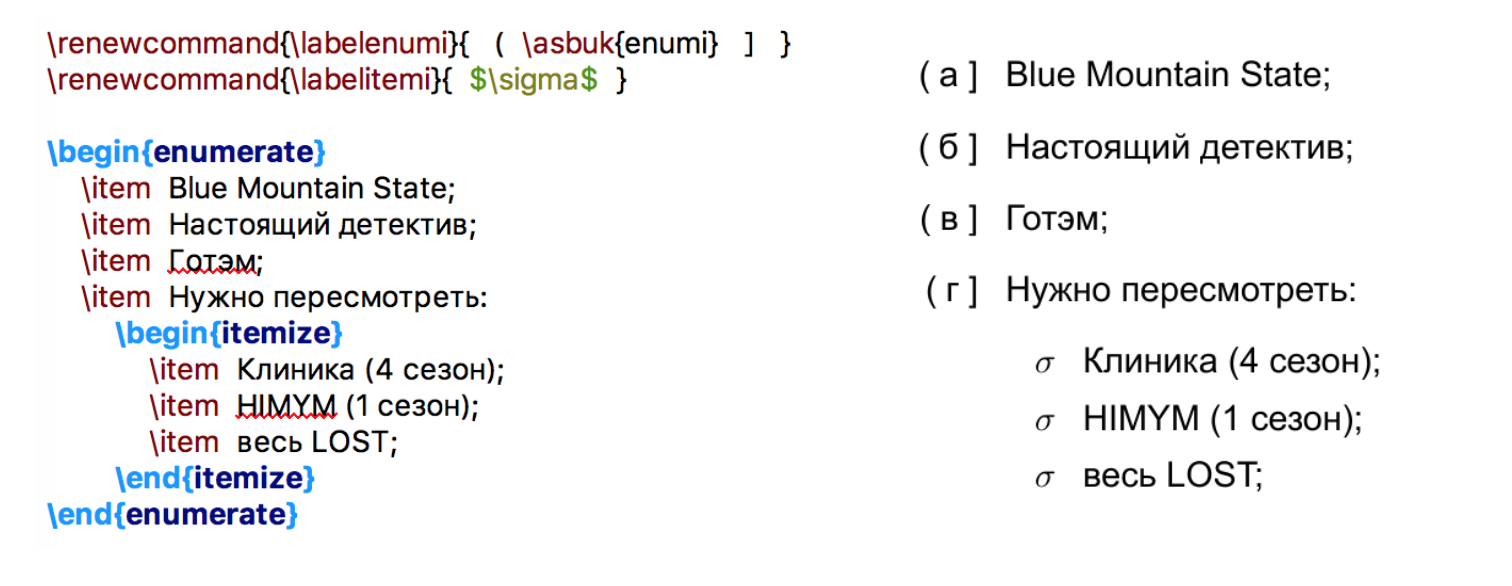
\includegraphics[scale=0.25]{ex2_2.png} 
\end{center}
\end{frame}


\begin{frame}{Пример 3: картинки}
\Large
\begin{block}{\Large Что мы хотим:}
	\begin{itemize}
		\item Вставить картинку
		\item Чтобы у неё была подпись и автоматическая нумерация 
	\end{itemize}
\end{block}
\end{frame}


\begin{frame}[fragile]{Пример 3: картинки}
\begin{tabular}{p{7cm}p{4cm}}
	\vspace{10mm} \verb|
\includegraphics[scale=0.15]{doge.png}| &  \begin{center} 
\includegraphics[scale=0.2]{doge.png} \end{center}
\end{tabular}
\end{frame}


\begin{frame}[fragile]{Пример 3: картинки}
\begin{center}
	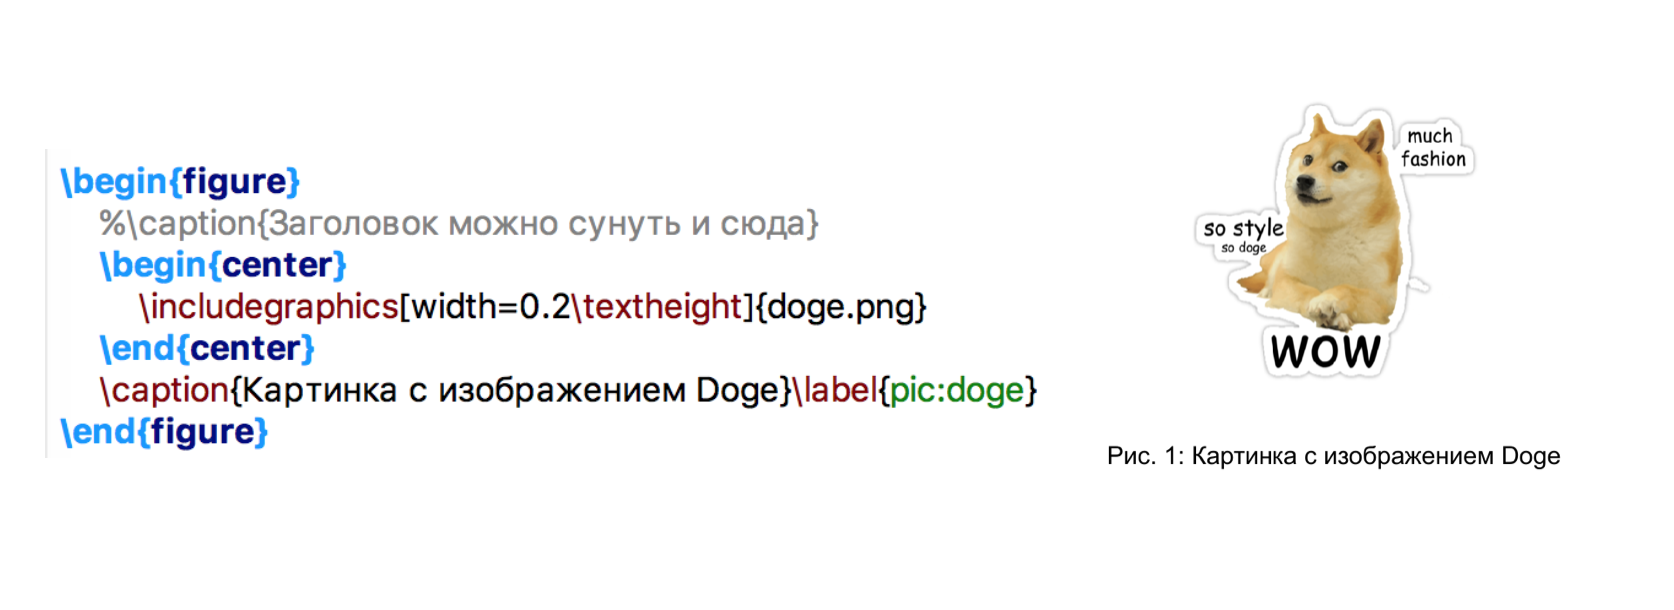
\includegraphics[scale=0.25]{ex3_1.png} 
\end{center}
\end{frame}


\begin{frame}[fragile]{Пример 3: картинки}
\begin{center}
	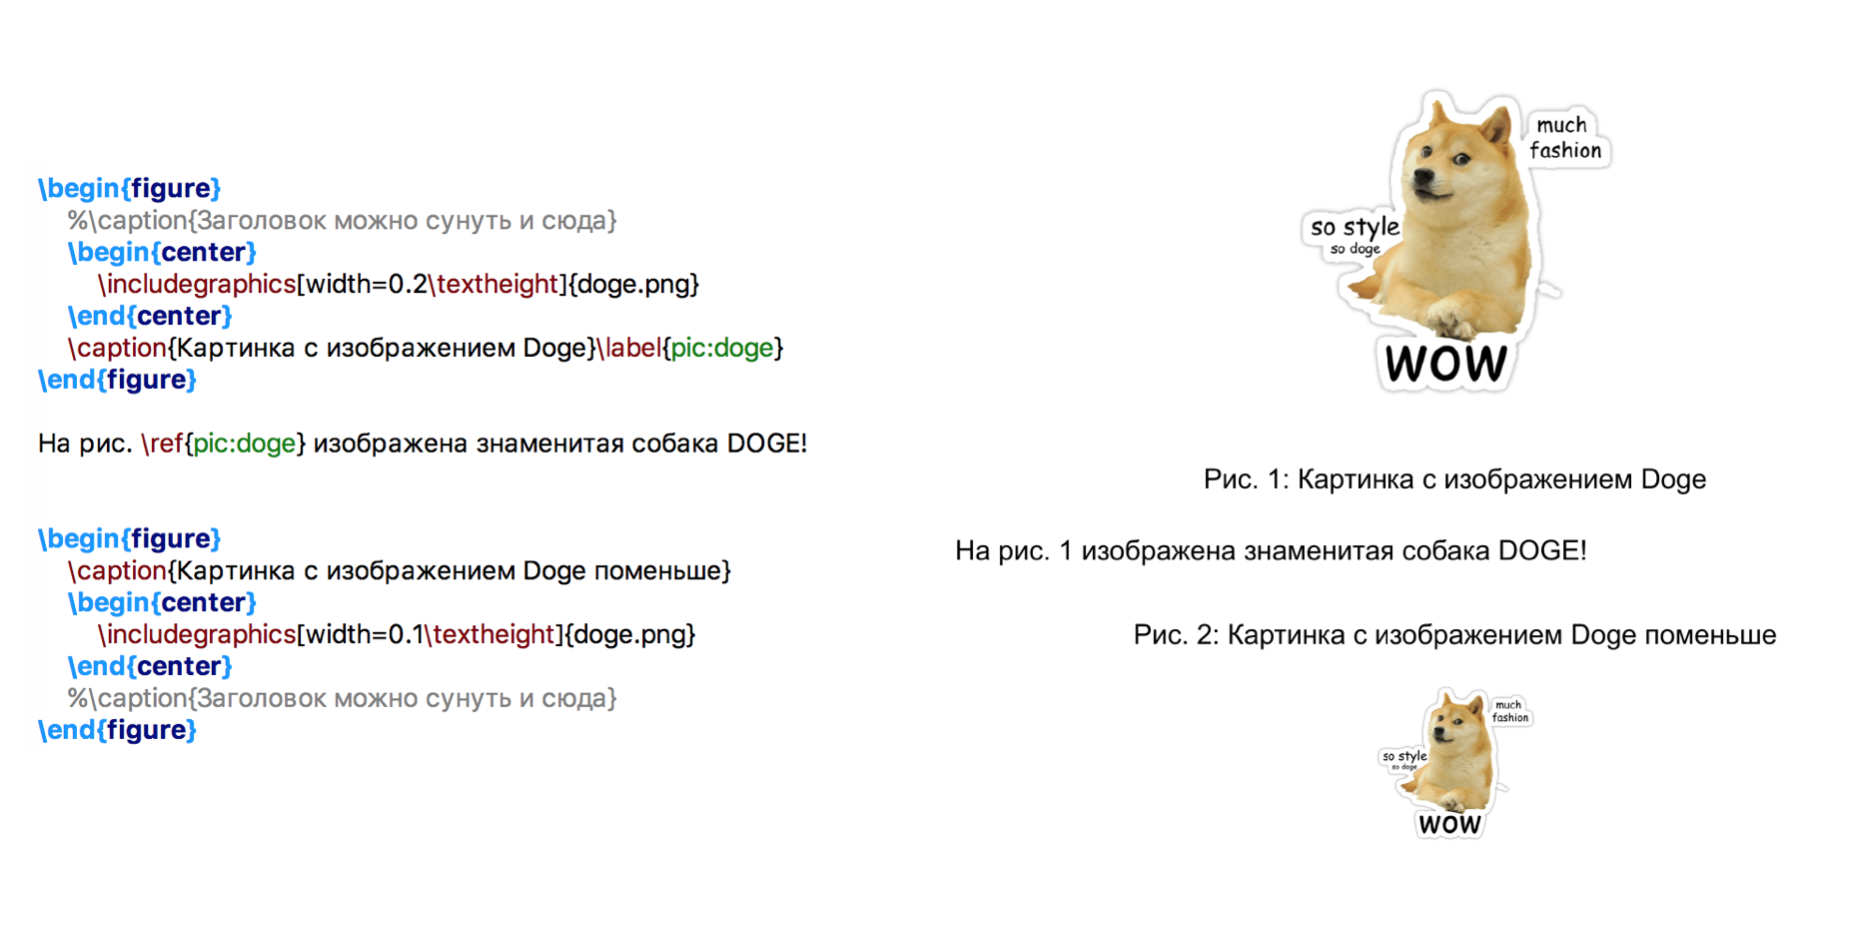
\includegraphics[scale=0.21]{ex3_2.png} 
\end{center}
\end{frame}


% показать проблему в теховском файле 
% показываем пакет по обузданию вольностей float и берём их под контроль

\begin{frame}{Пример 3: картинки}
\Large
\begin{block}{\Large Что мы хотим:}
	\begin{itemize}
		\item \LaTeX{ } думает, что знает лучше кожаных мешков где должна быть картинка, надо показать ему кто тут главный
	\end{itemize}
\end{block}
\end{frame}


\begin{frame}[fragile]
\begin{block}{Рисунок! Знай своё место!}
	\centering 
	\begin{tabulary}{\textwidth}{JL}
		\toprule
		с & поставить рисунок где удобно \TeX у и поместить его в центре (center) \\
		t & поставить рисунок где удобно \TeX у и прижать его к верху (top) \\
		b & поставить рисунок где удобно \TeX у и прижать его к низу   (bottom) \\
		p & поставить рисунок на отдельной странице, целиком состоящей из "плавающих" рисунков и таблиц \\
		h & поставить рисунок там, где он идет по тексту с нарушением всех правил верстки (here)  \\
		h! & поставить ну прям с высокой вероятностью там где надо нам \\
		H & в 100 случаях из 100 рисунок будет там где нам надо (нужно подгрузить пакет float) \\
		\bottomrule
	\end{tabulary}
\end{block}
\end{frame} 

\begin{frame}[fragile]{Пример 3: картинки}
\begin{center}
	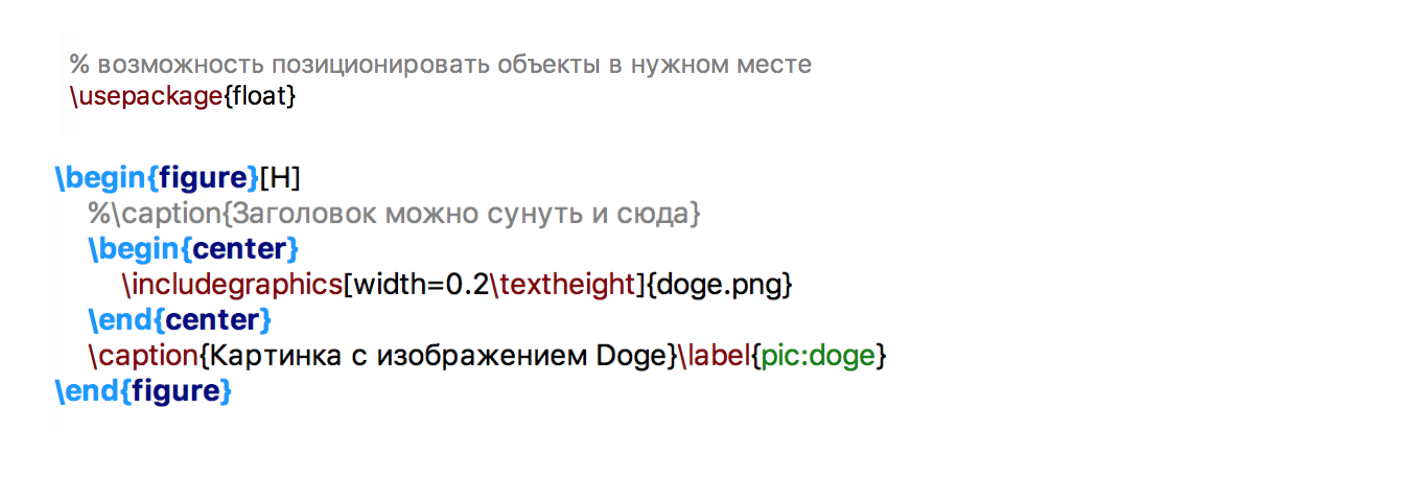
\includegraphics[scale=0.3]{ex3_3.png} 
\end{center}
\end{frame}


\begin{frame}{Пример 4: таблица}
\Large
\begin{block}{\Large Что мы хотим:}
	\begin{itemize}
		\item Вставить таблицу
		\item Чтобы у неё была подпись и автоматическая нумерация 
		\item Показать \LaTeX{ } что мы тут власть
	\end{itemize}
\end{block}
\end{frame}


\begin{frame}[fragile]{Пример 4: таблица}
\begin{center}
	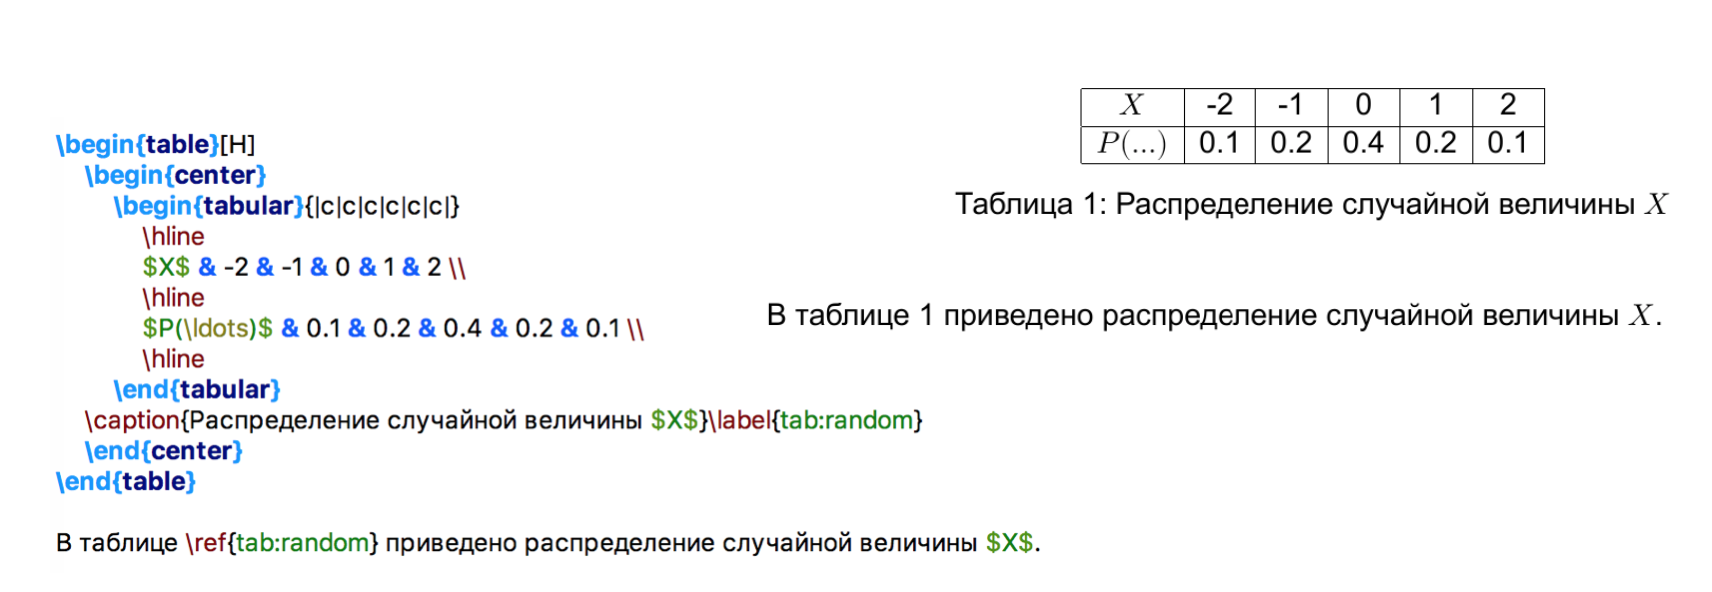
\includegraphics[scale=0.23]{ex4_1.png} 
\end{center}
\end{frame}


\begin{frame}{Мораль}
\begin{itemize}
	\item Основной объект в техе —  это окружение. Многие окружения уже заведены за нас, осталось только разобраться как они работают. 
	\item Мы можем заводить различные новые окружения. Например, если у нас есть два типа картинок, каждый из которых должен редактироваться по-своему, мы заведём для этого два разных окружения.
	\item Внутри документа мы делаем акцент на смысле. В преамбуле мы задаём оформление для разных окружений.
\end{itemize}
\end{frame}




\section{Мотивация ботать тех}

\begin{frame}{Сага о дипломе}
\centering
\alert{\textbf{Зачем первак, когда есть \LaTeX{}!}}


\includegraphics[height=0.68\textheight]{m4.png}
\end{frame}

%% Проблема 1: нумерация формул и сноски на них
\begin{frame}{Нумерация формул}
\centering
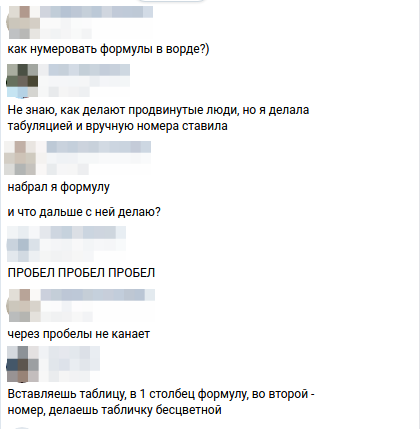
\includegraphics[scale=0.45]{pain.png}
\end{frame}


\begin{frame}{Нумерация формул}
\centering
\alert{\textbf{В \LaTeX{} все формулы нумеруются  автоматически!}}

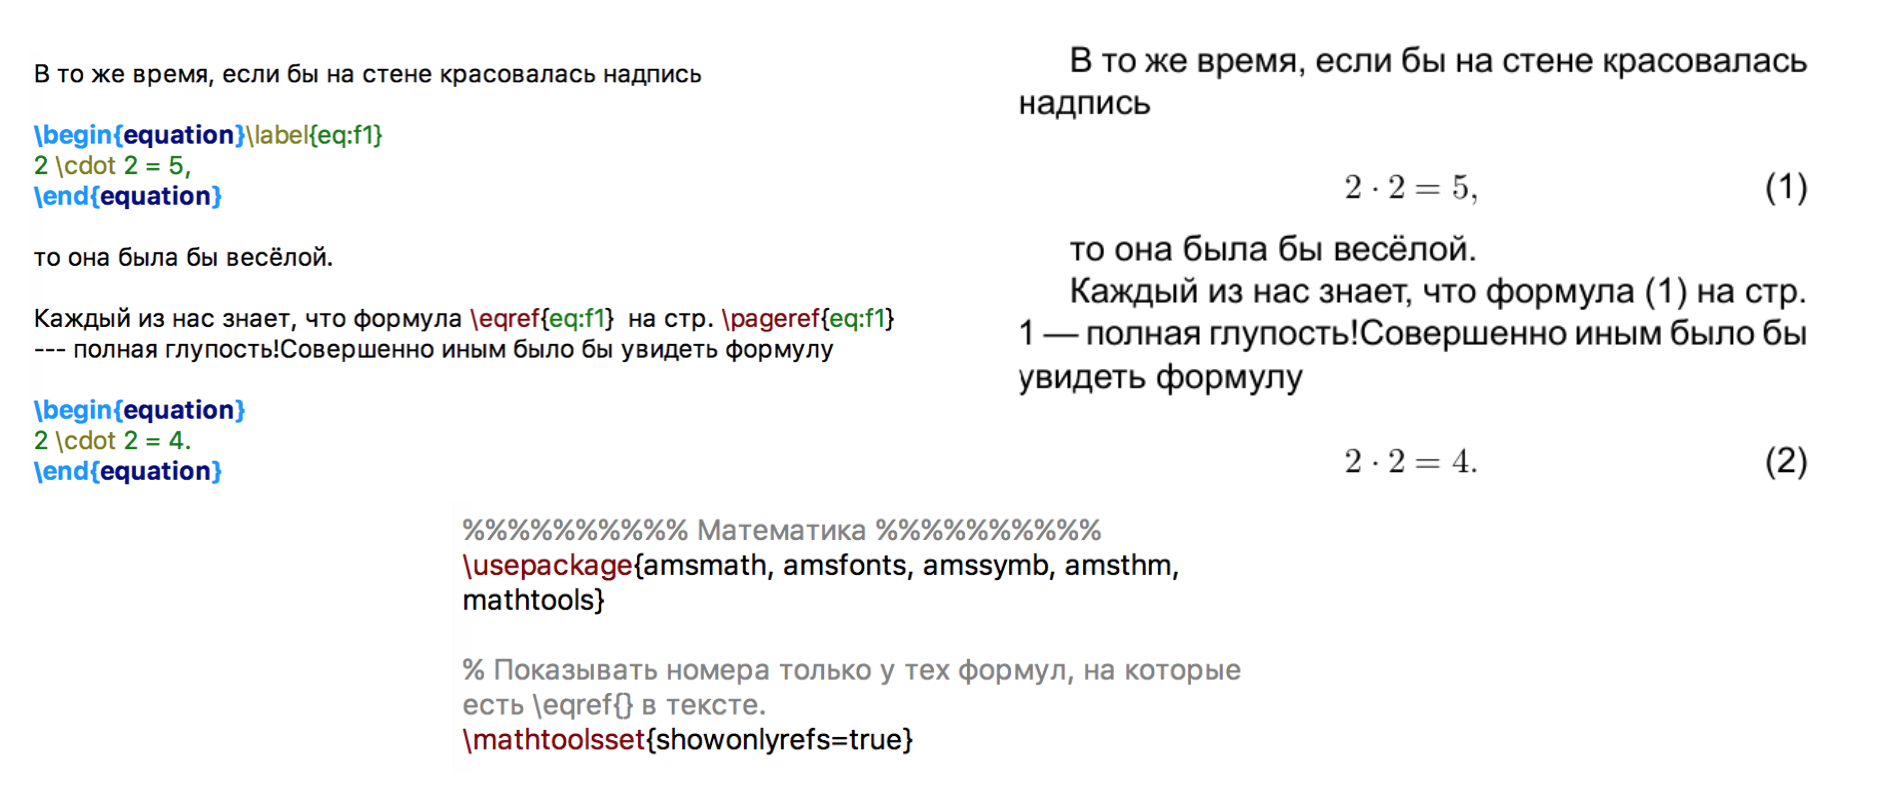
\includegraphics[width=0.98\linewidth]{document4.png}
\end{frame}


\begin{frame}{Автоматический список литературы}
   \centering
   \alert{\textbf{В \LaTeX{} список литературы сгенерируется автоматически!}}

    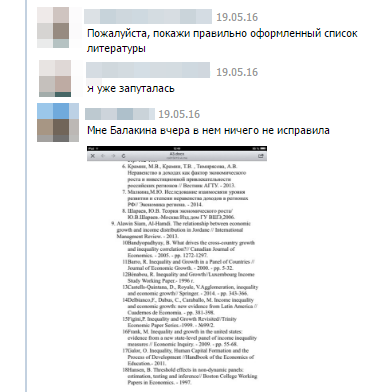
\includegraphics[height=0.95\textheight]{m2.png}
\end{frame}


\begin{frame}{Автоматическое оглавление}
\centering
\alert{\textbf{В \LaTeX{} оглавление сгенерируется автоматически!}}


\includegraphics[height=0.22\textheight]{m11.png}
\end{frame}


\begin{frame}{Всё съехало}
\centering

\includegraphics[scale=0.28]{word_pzd.jpg}

\vfill
\alert{\textbf{В \LaTeX{} ничего никогда не съедет!}}
\end{frame}


\begin{frame}{Что-то исчезло}
    \centering
    
\includegraphics[scale=0.2]{m7.png}

    \vfill
    \alert{\textbf{В \LaTeX{} ничего не изменится и не исчезнет без вашего ведома!}}
\end{frame}


\begin{frame}{Странные манипуляции}
    \centering
    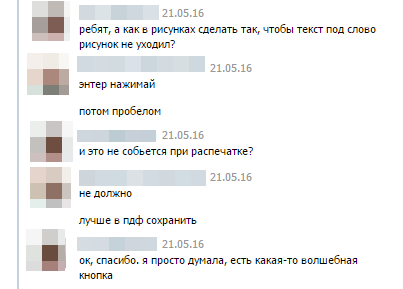
\includegraphics[height=0.6\textheight]{m6.png}

    \vfill
    \alert{\textbf{В \LaTeX{} вы навсегда забудете о "сначала энтер, потом 4 раза пробел"!}}
\end{frame}


\begin{frame}{ГОСТ-преамбула}
    \centering
    
\includegraphics[scale=0.8]{m5.png}

    \vfill
    \alert{\textbf{В \LaTeX{} можно написать абсолютно любой шаблон}}
\end{frame}



\begin{frame}
\centering
\alert{\textbf{\Large Это кусок чужого диплома, что тут не так?}}

\includegraphics[scale=0.2]{m228.jpg}
\end{frame}



\begin{frame}{А если говорить серьёзно, то \ldots}
    \centering
    \includegraphics[scale=0.2]{latexvsword.png}
\end{frame}



\begin{frame}{Точка пересечения слишком близко}
\centering
    \includegraphics[height=0.35\textheight]{tapaesh_probel.png}
\end{frame}


\begin{frame}{Если надо совсем простое}
\centering
    \includegraphics[scale=0.3]{markdown_vs_word.jpg}
\end{frame}


\section{Немного подробнее о математике в \LaTeX{}}



\begin{frame}{Почиташки}
\begin{itemize}
	\item  \href{https://www.mccme.ru/free-books/llang/newllang.pdf}{Книга Львовского.} Большая, очень подробная, ближе к середине есть много лишней информации для типографов. Её нужно проигнорировать.
	
	\item  \href{http://www.ccas.ru/voron/download/voron05latex.pdf}{Методичка Воронцова.} Куча примеров теховского кода и результатов его компиляции.
	
	\item  \href{https://ru.wikibooks.org/wiki/LaTeX}{Викиучебник по \LaTeX{.}}  Есть версия и на русском и на английском. Рекомендую смотреть интересующие вас сию секунду разделы. 
	
	\item  \href{https://www.overleaf.com/learn/latex/Creating_a_document_in_LaTeX}{Разные материалы от онлайн-сервиса Overliaf.} По аналогии с вики посмотрите какие разделы есть, смотрите их по необходимости.  
	
	\item \href{https://www.coursera.org/learn/latex}{Вышкинский курс на coursera.} Это для тех, кто хочет изучать \LaTeX, но не хочет ходить на пары. 
\end{itemize}
\end{frame}



%% СЛАЙД С КНИГАМИ ВИДЯХАМИ СТАТЬЯМИ  И ТП 

% книга львовского 
% методичка воронцова
% курс данилы (вас не трахнут)
% 
% 


\begingroup
\setbeamercolor{background canvas}{bg = LTXDarkGrey}
\begin{frame}[plain]
\vspace{0.5cm}
\centering \color{white}{\Huge{ KEEP CALM }}

\vspace{0.2cm}
\centering \includegraphics[width=0.7\linewidth]{joke_2.png}
\vspace{0.2cm}

\centering \color{white}{\Huge{ AND \TeX{ } IT }}
\end{frame}
\endgroup

\end{document}
